%% March 2018
%%%%%%%%%%%%%%%%%%%%%%%%%%%%%%%%%%%%%%%%%%%%%%%%%%%%%%%%%%%%%%%%%%%%%%%%%%%%
% AGUJournalTemplate.tex: this template file is for articles formatted with 
% LaTeX
%
% This file includes commands and instructions
% given in the order necessary to produce a final output that will
% satisfy AGU requirements, including customized APA reference formatting.
%
% You may copy this file and give it your
% article name, and enter your text.
%
%%%%%%%%%%%%%%%%%%%%%%%%%%%%%%%%%%%%%%%%%%%%%%%%%%%%%%%%%%%%%%%%%%%%%%%%%%%%
% PLEASE DO NOT USE YOUR OWN MACROS
% DO NOT USE \newcommand, \renewcommand, or \def, etc.
%
% FOR FIGURES, DO NOT USE \psfrag or \subfigure.
% DO NOT USE \psfrag or \subfigure commands.
%%%%%%%%%%%%%%%%%%%%%%%%%%%%%%%%%%%%%%%%%%%%%%%%%%%%%%%%%%%%%%%%%%%%%%%%%%%%
%
% Step 1: Set the \documentclass
%
% There are two options for article format:
%
% PLEASE USE THE DRAFT OPTION TO SUBMIT YOUR PAPERS.
% The draft option produces double spaced output.

%% To submit your paper:
\documentclass[draft,linenumbers]{agujournal2018}
\usepackage{apacite}
\usepackage{graphicx}
\usepackage[demo]{rotating}
\usepackage{url} %this package should fix any errors with URLs in refs.
\draftfalse 		% This option makes double space

%%%%%%%
% \usepackage{trackchanges}
% uncomment the line above to use the TrackChanges package to mark revisions 
% if needed.
% The trackchanges package adds five new LaTeX commands:
%
%  \note[editor]{The note}
%  \annote[editor]{Text to annotate}{The note}
%  \add[editor]{Text to add}
%  \remove[editor]{Text to remove}
%  \change[editor]{Text to remove}{Text to add}
%
% complete documentation is here: http://trackchanges.sourceforge.net/
%%%%%%%


% Now, type in the journal name: \journalname{<Journal Name>}

% ie, \journalname{Journal of Geophysical Research}
%% Choose from this list of Journals:
%
% JGR-Atmospheres
% JGR-Biogeosciences
% JGR-Earth Surface
% JGR-Oceans
% JGR-Planets
% JGR-Solid Earth
% JGR-Space Physics
% Global Biochemical Cycles
% Geophysical Research Letters
% Paleoceanography
% Radio Science
% Reviews of Geophysics
% Tectonics
% Space Weather
% Water Resource Research
% Geochemistry, Geophysics, Geosystems
% Journal of Advances in Modeling Earth Systems (JAMES)
% Earth's Future
% Earth and Space Science
% Geohealth
%

\journalname{Water Resource Research}

\begin{document}

%% ------------------------------------------------------------------------ %%
%  Title
% (A title should be specific, informative, and brief. Use
% abbreviations only if they are defined in the abstract. Titles that
% start with general keywords then specific terms are optimized in
% searches)
%% ------------------------------------------------------------------------ %%

% OPTION 1 - Antonio Preziosi
\title{Fine Sediment Deposition and Filtration: A Particle-Tracking 
Model Approach}

% OPTION 2 - Antonio Preziosi
% \title{Particle tracking model for kaolinite deposition in flumes under 
% losing or gaining flow conditions}

% OPTION 3 - Antonio Preziosi
% \title{Colloid exchange between a gaining/losing stream and streambed: 
% A particle tracking approach}

% Example: \title{This is a test title}

%% ------------------------------------------------------------------------ %%
%  AUTHORS AND AFFILIATIONS
%% ------------------------------------------------------------------------ %%

% Authors are individuals who have significantly contributed to the
% research and preparation of the article. Group authors are allowed, if
% each author in the group is separately identified in an appendix.)

% List authors by first name or initial followed by last name and
% separated by commas. Use \affil{} to number affiliations, and
% \thanks{} for author notes.
% Additional author notes should be indicated with \thanks{} (for
% example, for current addresses).

% Autores del paper
\authors{Antonio Preziosi-Ribero\affil{1}\thanks{Ciudad Universitaria,
Bogot\'{a}, Colombia}, Aaron I. Packman\affil{2}, Jorge A. Escobar-Vargas\affil{1, 3}, Colin B. Philips\affil{2} and Leonardo David Donado\affil{1}}

% Afiliaciones de los autores
\affiliation{1}{Universidad Nacional de Colombia, Facultad de Ingenier\'{i}a,
Bogot\'{a}, Colombia}
\affiliation{2}{Department of Civil and Environmental Engineering, 
Northwestern University, Evanston, IL, USA}
\affiliation{3}{Departamento de Ingenier\'{i}a Civil, Pontificia Universidad
Javeriana, Bogot\'{a}, Colombia}

% \affiliation{4}{Fourth Affiliation}

% \affiliation{=number=}{=Affiliation Address=}
%(repeat as many times as is necessary)

%% Corresponding Author:
% Corresponding author mailing address and e-mail address:

% (include name and email addresses of the corresponding author.  More
% than one corresponding author is allowed in this LaTeX file and for
% publication; but only one corresponding author is allowed in our
% editorial system.)

% Example: \correspondingauthor{First and Last Name}{email@address.edu}

\correspondingauthor{Antonio Preziosi-Ribero}{apreziosir@unal.edu.co}

%% Keypoints, final entry on title page.

% List up to three key points (at least one is required)
% Key Points summarize the main points and conclusions of the article
% Each must be 100 characters or less with no special characters or 
% punctuation

\begin{keypoints}
\item We developed a Particle-Tracking model for fine sediments' deposition taking into account free surface flow and groundwater input to a stream
\item Patterns of clay deposition depend on the velocity profile generated by the free surface flow conditions and groundwater vertical flow
\item Filtration process controls exclusively the deposition rate of particles in the domain, while the vertical flow controls the amount of particles inside it
\end{keypoints}

%% ------------------------------------------------------------------------ %%
%  ABSTRACT
% A good abstract will begin with a short description of the problem
% being addressed, briefly describe the new data or analyses, then
% briefly states the main conclusion(s) and how they are supported and
% uncertainties.
%% ------------------------------------------------------------------------ %%

\begin{abstract}
Fine particle deposition in rivers is an anomalous transport process and plays a major role in hyporheic exchange, riverine ecology and biogeochemistry. Indeed, this phenomenon is present in every stream or river at every stage of its flow. However, this phenomenon is poorly understood in river hydrodynamics and typical mathematical models and expressions like the Advection Dispersion Equation are not suitable to represent it accurately. To determine its extent, we developed a numerical Particle-Tracking (PT) model that simulates fine particles' deposition in an idealized sand dune under different steady vertical flow conditions (losing, neutral and gaining conditions). Later, we used previous experimental results from a clay deposition experiment in an experimental flume to assess qualitatively how accurate were our simulations. Our results suggest that fine particles' deposition patterns and residence time functions depend heavily on the groundwater flow conditions imposed and on the ability of the bed to trap the fine particles. In brief, our model was able to reproduce the experimental conditions supplying a framework to evaluate fine particles' deposition in sand beds, capturing the main physical processes involved and showing that Particle Tracking models are a suitable tool to represent anomalous transport processes with accurate results.  
\end{abstract}

% ============================================================================
% INTRODUCTION SECTION
% ============================================================================
\section{Introduction} \label{Introduction}

% 1. GENERAL PROBLEM AND HOW IT IS TREATED IN CURRENT LITERATURE
Fine sediment deposition is ubiquitous for all rivers and it is mainly driven by free surface flow conditions \citep{Packman2000,Packman2000b}. Nutrients and pollutants travel through the stream, get deposited in geomorphic controls like dunes, pools or ripples and return to the stream in different places. Along with sediment transport, this phenomenon has been fostered by land use changes in the latter times \citep{Wohl2015}, and both have effects in the biogeochemical processes as nutrient and carbon cycling \citep{Hope1994,Gottselig2014}, hence, the Hyporheic Exchange (HE).

Fine sediments are typically defined as minerals or organic particles packed in conglomerates with sizes smaller than $10\mu m$ \citep{Drummond2014,Drummond2018}. These particles are key drivers to processes like nutrient dynamics, carbon dynamics and contaminant transport. Moreover, they are well known for deposit in the stream bed and resuspend to the free flow with some periodicity \citep{Drummond2015} depending on the surface flow driven by extreme events like storms \citep{Drummond2017}. However, their retention in the stream bed is known to affect hyporheic flow, exchange of nutrients and physical properties of the media like porosity and permeability. 

% 2. WHAT IS MISSING FROM THE APPROACH THAT HAS BEEN TAKEN SO FAR
Current literature about HE and sediment deposition relays on experiments and observations in field scale, laboratory flumes and numerical models \citep{Salehin2004a,Marion2002,Fox2014,Fox2018}. For the laboratory scale experiments, recirculating flumes with sand beds are used along with dissolved clay, e.g. Kaolinite, to assess its deposition with photographs and dye injections \citep{Fox2014,Fox2018}. Instead, in the field scale, the concentration of fine particles is quantified in different river beds during baseflow and after storm flows \citep{Drummond2017}. As regards to numerical models, the use of the Advection Dispersion Equation (ADE) has been used to estimate solute transport \citep{Boano2007b,BayaniCardenas2008c}, and particle tracking models for estimating deposition under steady conditions that only depend on the surface flow \citep{Packman2000}. 

Nowadays, understanding of complex phenomena like fine sediments' deposition can be tackled using lagrangian models \citep{Schumer2009}, that do not rely on continuum equations and typical discretization schemes, i.e. finite elements, volumes or differences \citep{Noetinger2016}. However, current literature lacks of numerical models able to estimate fine sediment deposition taking into account the conditions of the groundwater flow beneath the stream.

% 3. WHAT IS THE PROPOSED MODEL AND HOW IT WILL SOLVE THIS LACK OF INFORMATION
Therefore, the goal of this study was to implement a numerical particle-tracking model for fine sediments' deposition that takes into account both, free surface flow and subsurface vertical flow, assuming a losing, neutral or gaining condition for the stream. The set up is inspired in the work by \citet{Fox2014,Fox2018}, and the numerical Particle-Tracking (PT) model is used to estimate fine sediments' deposition patterns using simple rules under the different flow conditions. Later, our results are compared with the flume experiments to asses how a complex phenomenon like fine particles' deposition is represented by a discretized PT model. 

% 4. WHAT ARE THE RESULTS BROADLY SPEAKING
The implementation of the PT tracking model for fine particles' deposition in the subsurface domain of a single dune used steady velocity profiles generated from the superposition of subsurface flow generated by the Advective Pumping Model (APM) \citep{Elliott1997,Elliott1997b}, and three different vertical flow conditions, i.e. losing, neutral and gaining flow. Sediment particles move with the streamlines and are trapped inside the domain using a stochastic function, hence simulating the adhesion of clay to the sand in the riverbed \citep{Li2017}. Our results show that the model captures the main physical phenomena present in the fine sediments' deposition in an idealized homogeneous media. Besides, it foster the basic understanding of the sediments' deposition process in more complex media like flumes and rivers.

After the results are presented, they are compared qualitatively with the experimental results from \citet{Fox2014,Fox2018}, to assess the model performance in respect to a real experimental case with proven results. Broadly, the numerical model is able to represent the mean behavior of the clay deposition phenomenon and the PT model is able to represent the complex clay deposition pattern in the physical experiments performed. 

% ============================================================================
% METHODS SECTION
% ============================================================================
\section{Methods} \label{Methods}

\subsection{Conceptual model} \label{Conceptual_Model}

% The conceptual model and how particles move in the domain
Our particle tracking model aims to represent fine sediments' deposition in an idealized sand-bed (figure \ref{Conceptual}). It is inspired in the experimental setup that has been used by different authors \citep{Elliott1997b,Elliott1997b,Packman2000b,Fox2014,Fox2018}, but in our case a gaining or losing flux is imposed at the bottom of the domain to assess the way vertical flow affects clay deposition, and consequently, hyporheic flow. As a consequence, the initial conditions of the numerical model are closely related with the experiments on clay deposition values reported in literature \citep{Packman2000,Fox2014,Fox2018}, and shown in table \ref{TF:Phys_Param}. Nevertheless, to generalize the model, non dimensional quantities are used for the comparisons.

% ============================================================================
% Conceptual model of the problem proposed - figure
\begin{figure}[ht]
\centering
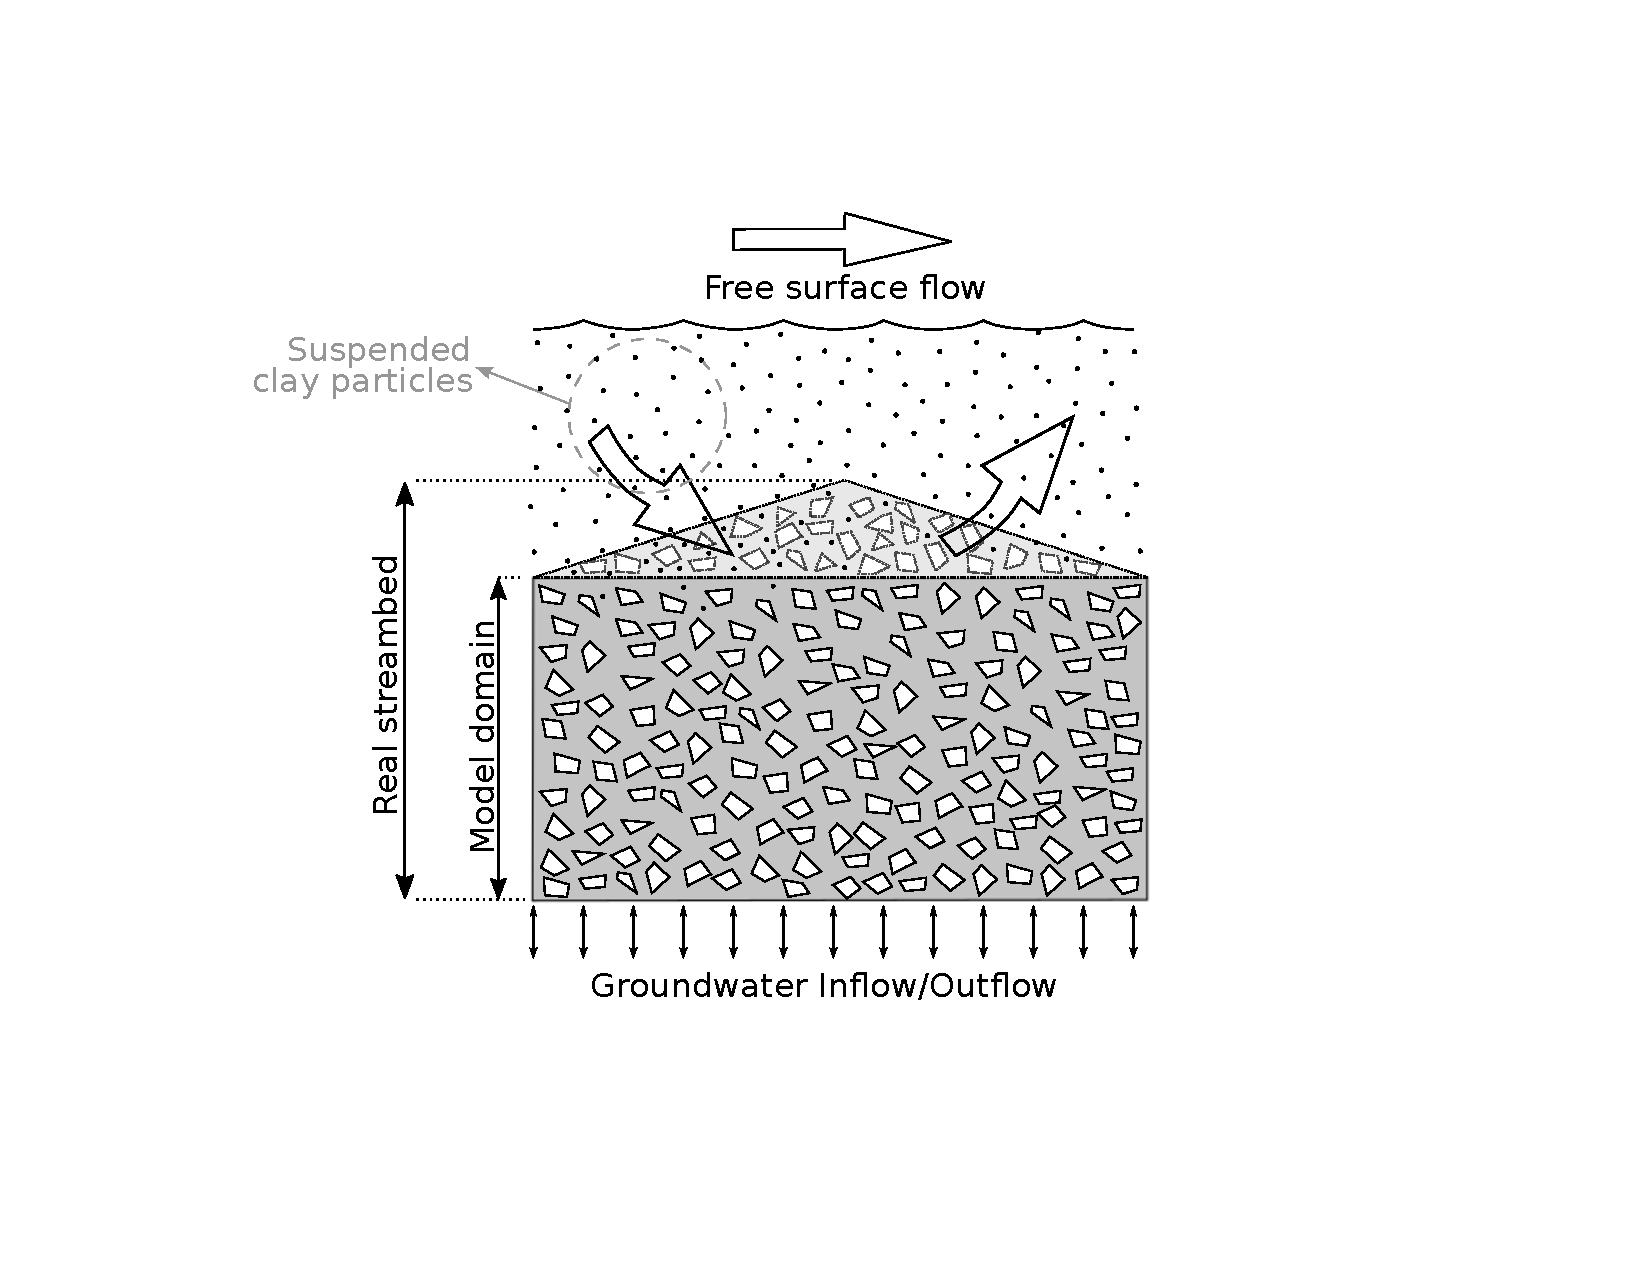
\includegraphics[clip, trim=4.2cm 4.5cm 8cm 3cm, width=28pc]
{1807010Conceptual.pdf}
\caption{Conceptual model for the posed problem. The dune shape is replaced by a pressure head over the dune, hence the numerical model is a rectangular box. The inflow/outflow conditions are imposed at the bottom of the domain.}
\label{Conceptual}
\end{figure}
% ============================================================================

% ============================================================================
% TABLE WITH PHYSICAL AND NUMERICAL PARAMETERS FOR THE PARTICLE-TRACKING
% MODEL THAT WAS PROPOSED
% ============================================================================
\begin{table}
\caption{Physical parameters \citep{Packman2000,Fox2014,Fox2018} for the comparison of the Particle-Tracking model implemented.}
\label{TF:Phys_Param}
\centering
\begin{tabular}{l c c}
\hline
PHYSICAL PARAMETERS						& SYMBOL			& VALUE			\\
\hline
  Flume width $[cm]$  					& $W$				& 29.0 			\\
  Sediment porosity $[-]$				& $\theta$			& 0.33 			\\
  Hydraulic conductivity $[cm/s]$ 		& $K$				& 0.12 			\\
  Flow $[l/min]$						& $Q$				& 261.0			\\
  Mean stream velocity $[cm/s]$			& $U$				& 15.0 			\\
  Streambed depth $[cm]$				& $d_b$				& 20.0 			\\
  Dune wavelegth $[cm]$					& $\lambda$			& 15.0 			\\
  Water depth $[cm]$					& $d$				& 8.8 			\\
  Total streambed area $[cm^{2}]$		& $A$				& 15.1	 		\\
  Inflow/Outflow$^{b}$ $[cm/d]$			& $q_{in}$			& $\pm 12.5$	\\
  Filtering coefficient $[1/cm]$		& $\lambda_f$		& 0.6			\\
\hline
\multicolumn{2}{l}{$^{a}$All units in $cgs$ system for convenience} \\
\multicolumn{2}{l}{$^{b}$Positive quantities point upwards, negative 
downwards} \\
\end{tabular}
\end{table}
% ============================================================================

The main assumptions of our model are (i) the shape of the dunes and clay's behavior inside the dunes of the flume is fairly similar and repetitive \citep{Vanoni1974}, hence a single dune is enough to represent the behavior of a system of $n$ consecutive bedforms; (ii) particles do not interact with each other and they do not change the flow conditions in the media when they are trapped in the bed; and (iii) a trapped particle will not move any more after the moment it has been trapped by the media.

The initial condition of the model is an instantaneous injection of particles at the left half of the top boundary of the model domain, then for every timestep particles move according to an estimated 2D velocity profile and a stochastic function will determine if they are trapped in the place they moved to. Sections \ref{Mathematical_model} and \ref{Numerical_model} will explain in depth the moving and trapping/filtering features of the model. 

\subsection{Mathematical Model} \label{Mathematical_model}

The velocity profiles used for modeling the water flow inside the dune are taken from existing literature \citep{Elliott1997,Packman2000} and are illustrated in equations \ref{u} and \ref{v}. Nonetheless, the groundwater vertical flow condition is added to the existing profiles (i.e. positive upwards velocity for gaining condition and negative downwards velocity for the losing condition). Here, $x$ and $y$ are the Cartesian coordinates reference axis, $k$ stands for the normalized dune wavelength $(2 \pi / \lambda)$ and $u$ and $v$ for the horizontal and vertical velocity components, respectively. Futhermore, $h_m$ represents the mean pressure over the dune, $K$ stands for the permeability of the media, $d_b$ for the thickness of the bed that is analyzed and $q_{in/out}$ is the component of vertical velocity caused by the groundwater inflow/outflow. 

% Velocity profile equations - From Packman et al. 2000
% use \nonumber if you want to split an equation in different rows and not number a row
\begin{eqnarray}
\label{u}
  u & = & -(kKh_{m}) \cos(kx) [\tanh(kd_b)\sinh(ky) + \cosh(ky)] \\
\label{v}
  v & = & -(kKh_{m}) \sin(kx) [\tanh(kd_b)\cosh(ky) + \sinh(ky)] \pm q_{in/out} 
\end{eqnarray}

All of the quantities are normalized according to the theory developed for flow and transport in sand beds \citep{Elliott1997,Packman2000}. As a result, equations \ref{u} and \ref{v} can be transformed in equations \ref{ustar} and \ref{vstar}. The inflow/outflow velocity $q_{in/out}$ is normalized with the maximum punping velocity $u_m$. The resulting velocity profiles (figure \ref{Velocities}), exhibit how the addition of the vertical velocity shifts preferential flow direction and highlights the places where flow recirculation is present (figure \ref{Velocities}a and \ref{Velocities}c).  

% Dimensionless velocity profiles - From Packman with Elliott 
\begin{eqnarray}
\label{ustar}
  u^* & = & -\cos(x^*)[\tanh(d_b^*)\sinh(y^*) + \cosh(y^*)]\\
\label{vstar}
  v^* & = & -\sin(x^*)[\tanh(d_b^*)\cosh(y^*) + \sinh(y^*)] \pm q_{in/out}^*
\end{eqnarray}

The velocity component that corresponds to the settling velocity in previous papers \citep{Packman2000} was neglected for this model since the Stokes number of the particle is close to zero, thus particle will follow the streamlines of the velocity profiles generated by equations \ref{u} and \ref{v} \citep{Clark2009}. Equation \ref{STK} shows the calculation of the Stokes number for clay particles moving in porous media with representative length and velocity. 

% Stokes number calculation
\begin{equation}
 \label{STK}
 	Stk = \frac{\rho_p d_p^2 u_0}{18 \mu_f l_0} = \frac{2650 \frac{kg}{m^3} \cdot [384 \times 10^{-6}m]^2 \cdot 0.01 \frac{m}{s}}{18 \cdot 1.519 \times 10^{-3}Pa \ s \cdot 0.01 m} = 0.014
 \end{equation}

Where $\rho_p$ stands for the typical density of kaolinite \citep{NationalCenterforBiotechnologyInformation}, $d_p$ is the mean particle diameter \citep{Fox2014}, $u_0$ is the mean velocity, which is taken to be greater than the maximum obtained from equations \ref{u} and \ref{v}, $\mu_f$ is water's dynamic viscosity \citep{Cengel2006}, and $l_0$ is the characteristic length of the phenomenon which is similar to the dune height \citep{Fox2018}. The value of the stokes number is less than 1.0, i.e. a clay particle will follow the streamlines of the velocity profile without diverging from them \citep{Tropea2007}.

% ============================================================================
% Velocity profiles - figure
\begin{figure}[ht]
\centering
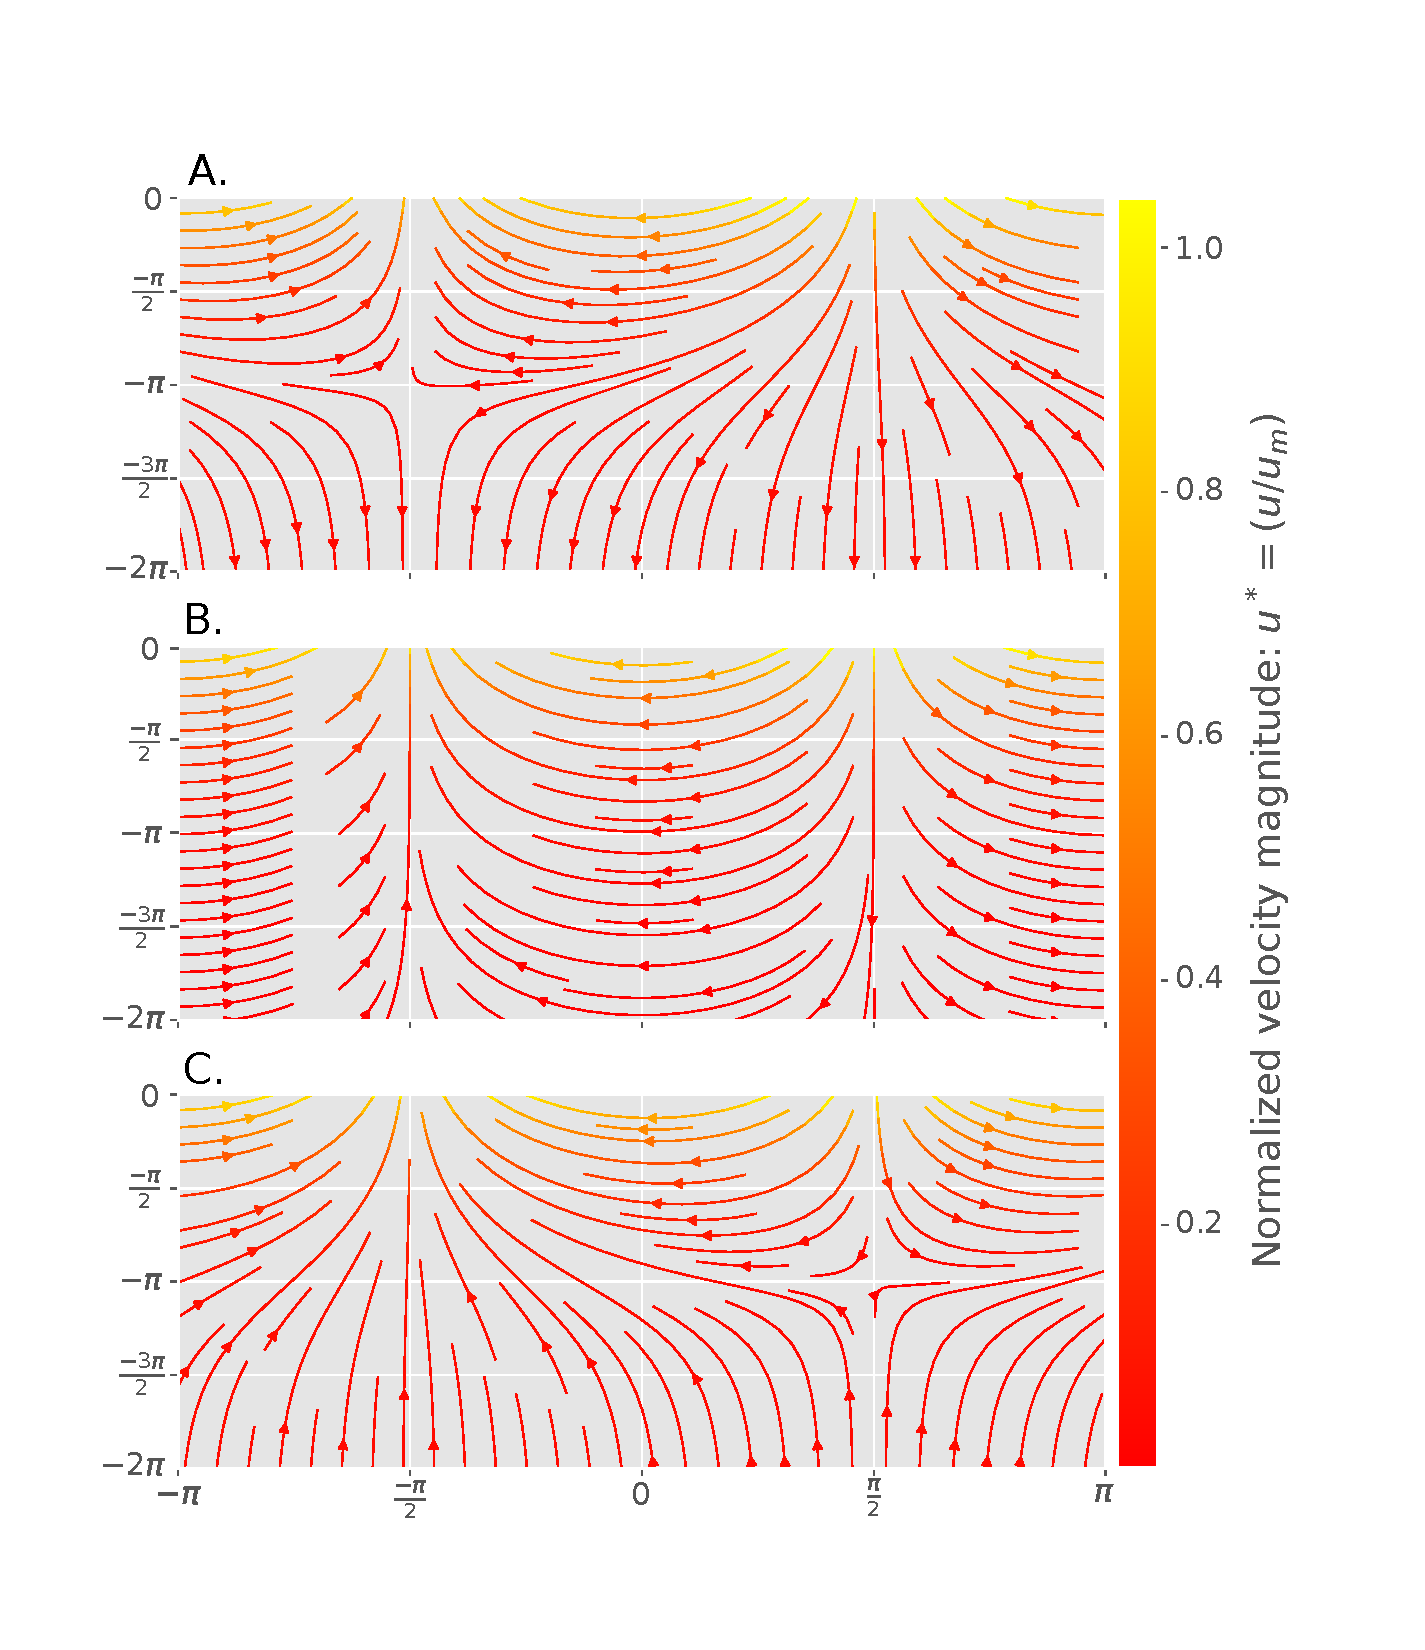
\includegraphics[trim=2cm 1.5cm 4cm 0.1cm, width=35pc]
{190131_Streamlines.pdf}
\caption{Streamlines plot under different vertical flow conditions: (A) Losing, (B) Neutral and (C) Gaining. Plots' domains are shifted from $[0, 2 \pi]$ to $[-\pi /2, \pi/2]$ since domain is periodic. The color bar points the magnitude of the velocity vector. Note that the vertical scale is distorted.}
\label{Velocities}
\end{figure}
% ============================================================================

The modeled clay particles follow the streamlines formed by the velocity profiles described in equations \ref{ustar} and \ref{vstar}. They are not a solute, i.e. they don't take into account diffusive processes \citep{Domenico1998}. As a consequence, the particles' transport is composed by the advection caused by the velocity profile and the effects of filtration that have to be included as a stochastic process over each particle that is simulated at the end of every time step \citep{Prickett1981}. 

Consequently, the standard Advection Dispersion Equation is transformed into a transport equation that takes into account only the advection process as depicted in equation \ref{ADE}. Namely, in the continuum an advection process will move a concentration front with a given velocity profile. For the case of this research, the velocity profiles are the ones given in equations \ref{ustar} and \ref{vstar}.

% Advection Dispersion Equation with just advection!!!!
\begin{equation}
 \label{ADE}
 	\frac{\partial C}{\partial t} \ = -u \frac{\partial C}{\partial \bar{x}}
 \end{equation}

The second part of the model accounts for filtration, which is modeled as a first-order process that depends on the path traveled by a particle, as shown in equation \ref{Filt_cont}. Where $\lambda_f$ denotes the filtration coefficient between 0.0 and 1.0, and $s$ the distance traveled by a single particle in the concentration front. Correspondingly, the proposed filtration process is dependent on the path traveled by each particle. 

% Concentration reduction due to filtration of particles (equation)
 \begin{equation}
 \label{Filt_cont}
 	\frac{\partial C}{\partial s} \ = -\lambda_f C
 \end{equation}

\subsection{Numerical Model} \label{Numerical_model}

The numerical model proposed is similar to the one used by \citet{Packman2000}. Its logical process is divided in three parts that use the discrete versions of equations \ref{ADE} and \ref{Filt_cont}. These versions have been proposed in the literature \citep{Delay2005,Dentz2011}, following a modified version of the Langevin equation, suited to represent in a discrete way the ADE including reaction process. The codes for the model are available at \citep{Preziosi2019}.

The first step takes into account the initial position of each particle and calculates the displacement of particles using equations \ref{dispx} and \ref{dispy} \citep{Li2017}. Hence, each timestep the model takes into account the previous position of each particle and interpolates the velocity fields to determine its velocity at the point where it is. As it was mentioned in the main assumptions of section \ref{Methods}, collision between particles or conglomeration are not taken into account. 

% Particle displacement for the "first step" of the numerical model
\begin{eqnarray}
 \label{dispx}
 	x(t + \Delta t) = x(t)  + u \cdot \Delta t\\
 \label{dispy}
 	y(t + \Delta t) = y(t) + v \cdot \Delta t
 \end{eqnarray}
 
In non dimensional form, each particle's displacement is estimated by:

% Particle displacement for the "first step" of the numerical model
\begin{eqnarray}
 \label{dispx_s}
 	x^*(t^* + \Delta t^*) = x^*(t^*)  + u^* \cdot \Delta t^*\\
 \label{dispy_s}
 	y^*(t^* + \Delta t^*) = y^*(t^*) + v^* \cdot \Delta t^*
 \end{eqnarray}
 
After estimating each particle's position, the discrete filtration process is modeled using a uniform random number generator inside the script. To do so, the filtration coefficient is taken as each  particle's probability $p$ of being filtered given that it traveled a distance $\Delta s = \sqrt{x^2 + y^2}$. Therefore, equation \ref{Filt_cont} is translated to the discrete domain using equation \ref{Filt_disc}, since the timestep size is small enough to hold the relationship posed in the right hand side of equation \ref{Filt_disc} \citep{Li2017}.
 
 % Simplification of the continuum - from eulerian to particles
 \begin{equation}
 \label{Filt_disc}
 	p = 1 - e^{-\lambda_f \Delta s} \approx \lambda_{f} \Delta s
 \end{equation}

The end of every timestep consists of counting the amount of particles that are still in the domain, which is divided in filtered particles that will remain still for the rest of the simulation; and moving particles, which have not been filtered yet. Besides, the model accounts for the particles that went out of the domain because of their recirculation to the stream. Particularly, the particles that recirculate every timestep are not allowed to come back to the sand bed any more. 

To ensure that the computational domain of the model is representative of a single dune, the boundary conditions at the right and left walls of the model are periodic. Namely, a particle that has an $x^* < 0$ will appear at the right of the domain. Correspondingly, a particle's $x^* > 2 \pi$ is transferred to the left part of the domain. Regarding the bottom boundary, any particle whose $y^* < d_b^*$ bounces inside the domain. On the other hand, any particle whose $y^* > 0$ is counted as recirculated and exits the simulation. 

The particle-tracking simulations were performed under similar conditions to the ones proposed in table \ref{TF:Phys_Param} with $1x10^5$ and $2x10^5$ particles for each vertical flow condition imposed (Losing, Neutral and Gaining). The total time simulated ensured that all of the seeded particles were recirculated or filtered by the end of the simulation. Nonetheless, the clay injection proposed in the numerical model is instantaneous and not continuous as in the experimental set-up. 

As regards to the initial condition, the particles are seeded evenly distributed at the top of the domain and just in the left portion of it ($0 < x^* < \pi$), since particles seeded at the right part of the domain ($\pi < x^* < 2\pi$) will immediately be recirculated due to the velocity profiles provided for the particle flow, as shown in figure \ref{Velocities}. At the end of every simulation, the results are two tables with coordinates of filtered and moving particles for every timestep, and a vector that counts the recirculated particles in the different timesteps. 

% About the relative concentration windows where the results are analyzed.
These raw results are then grouped to get information that is comparable with experimental results. Hence, the model's domain is divided into $\pi / 50$ side squares and then particles are counted every timestep recorded to get the relative concentration in the grid of the model. The domain division is independent from the interpolation points used for the velocity interpolation.

Selecting the mesh size for the particle counting is not trivial and in this case, different sizes of mesh were tested. If the mesh is coarse, the results will not be able to represent the phenomenon, and if the mesh size approaches to zero, the number of particles in every cell will not be representative of the phenomenon that is being modeled \citep{Xue2017}. In addition, methods like kernel density estimation (KDE), are not explored here since this is not the scope of this research. 

% ============================================================================
% RESULTS SECTION
% ============================================================================
\section{Results}  \label{Results}

% 0. VELOCITY PROFILES UNDER DIFFERENT CONDITIONS WHEN SOLVING FOR THE DIFFERENT IN/OUT VALUES
The velocity profiles that result from equations \ref{ustar} and \ref{vstar} (figure \ref{Velocities}) show substantial differences among them. Indeed, there is a preferential flow going upwards or downwards if the imposed condition is a gaining or losing flow, respectively. Furthermore, there is a no flow zone in the losing and gaining conditions formed by the addition of a vertical flow to a neutral flow condition. Consequently, there is a recirculation zone in the losing and gaining cases, though they are in different places according to the case. Namely, in the gaining condition it is located in the right part of the domain, while for the losing condition it is located at the left.

Furthermore, the maximum velocity in each profile is located in a different place. In particular, in the losing condition the maximum velocity is in the negative direction at the stoss side of the domain, while in the gaining case it is located in dune's lee. However, for the neutral condition there are two maximum velocities, one located in the stoss and the second in the lee. These features that the velocity profiles exhibit are key to understand the deposition of particles inside the domain when running the PT model, and they are the responsible of the different deposition patterns that result.   

% 1. PARTICLE DEPOSITION OVER DIFFERENT TIMES AND DIFFERENT CONDITIONS (COMPARE BETWEEN THEM) - explain the plots
The portion of particles deposited inside the domain evolves in time differently for the three conditions modeled (figure \ref{Logmap}). Each column of this figure corresponds to a flow condition modeled and on each row a different time is plotted for each one of the aforementioned conditions. This kind of plot was selected over a normal concentration plot since the places with no particles can be spotted easily. 

% ============================================================================
% Logarithm of concentration - figure
\begin{sidewaysfigure}
\centering
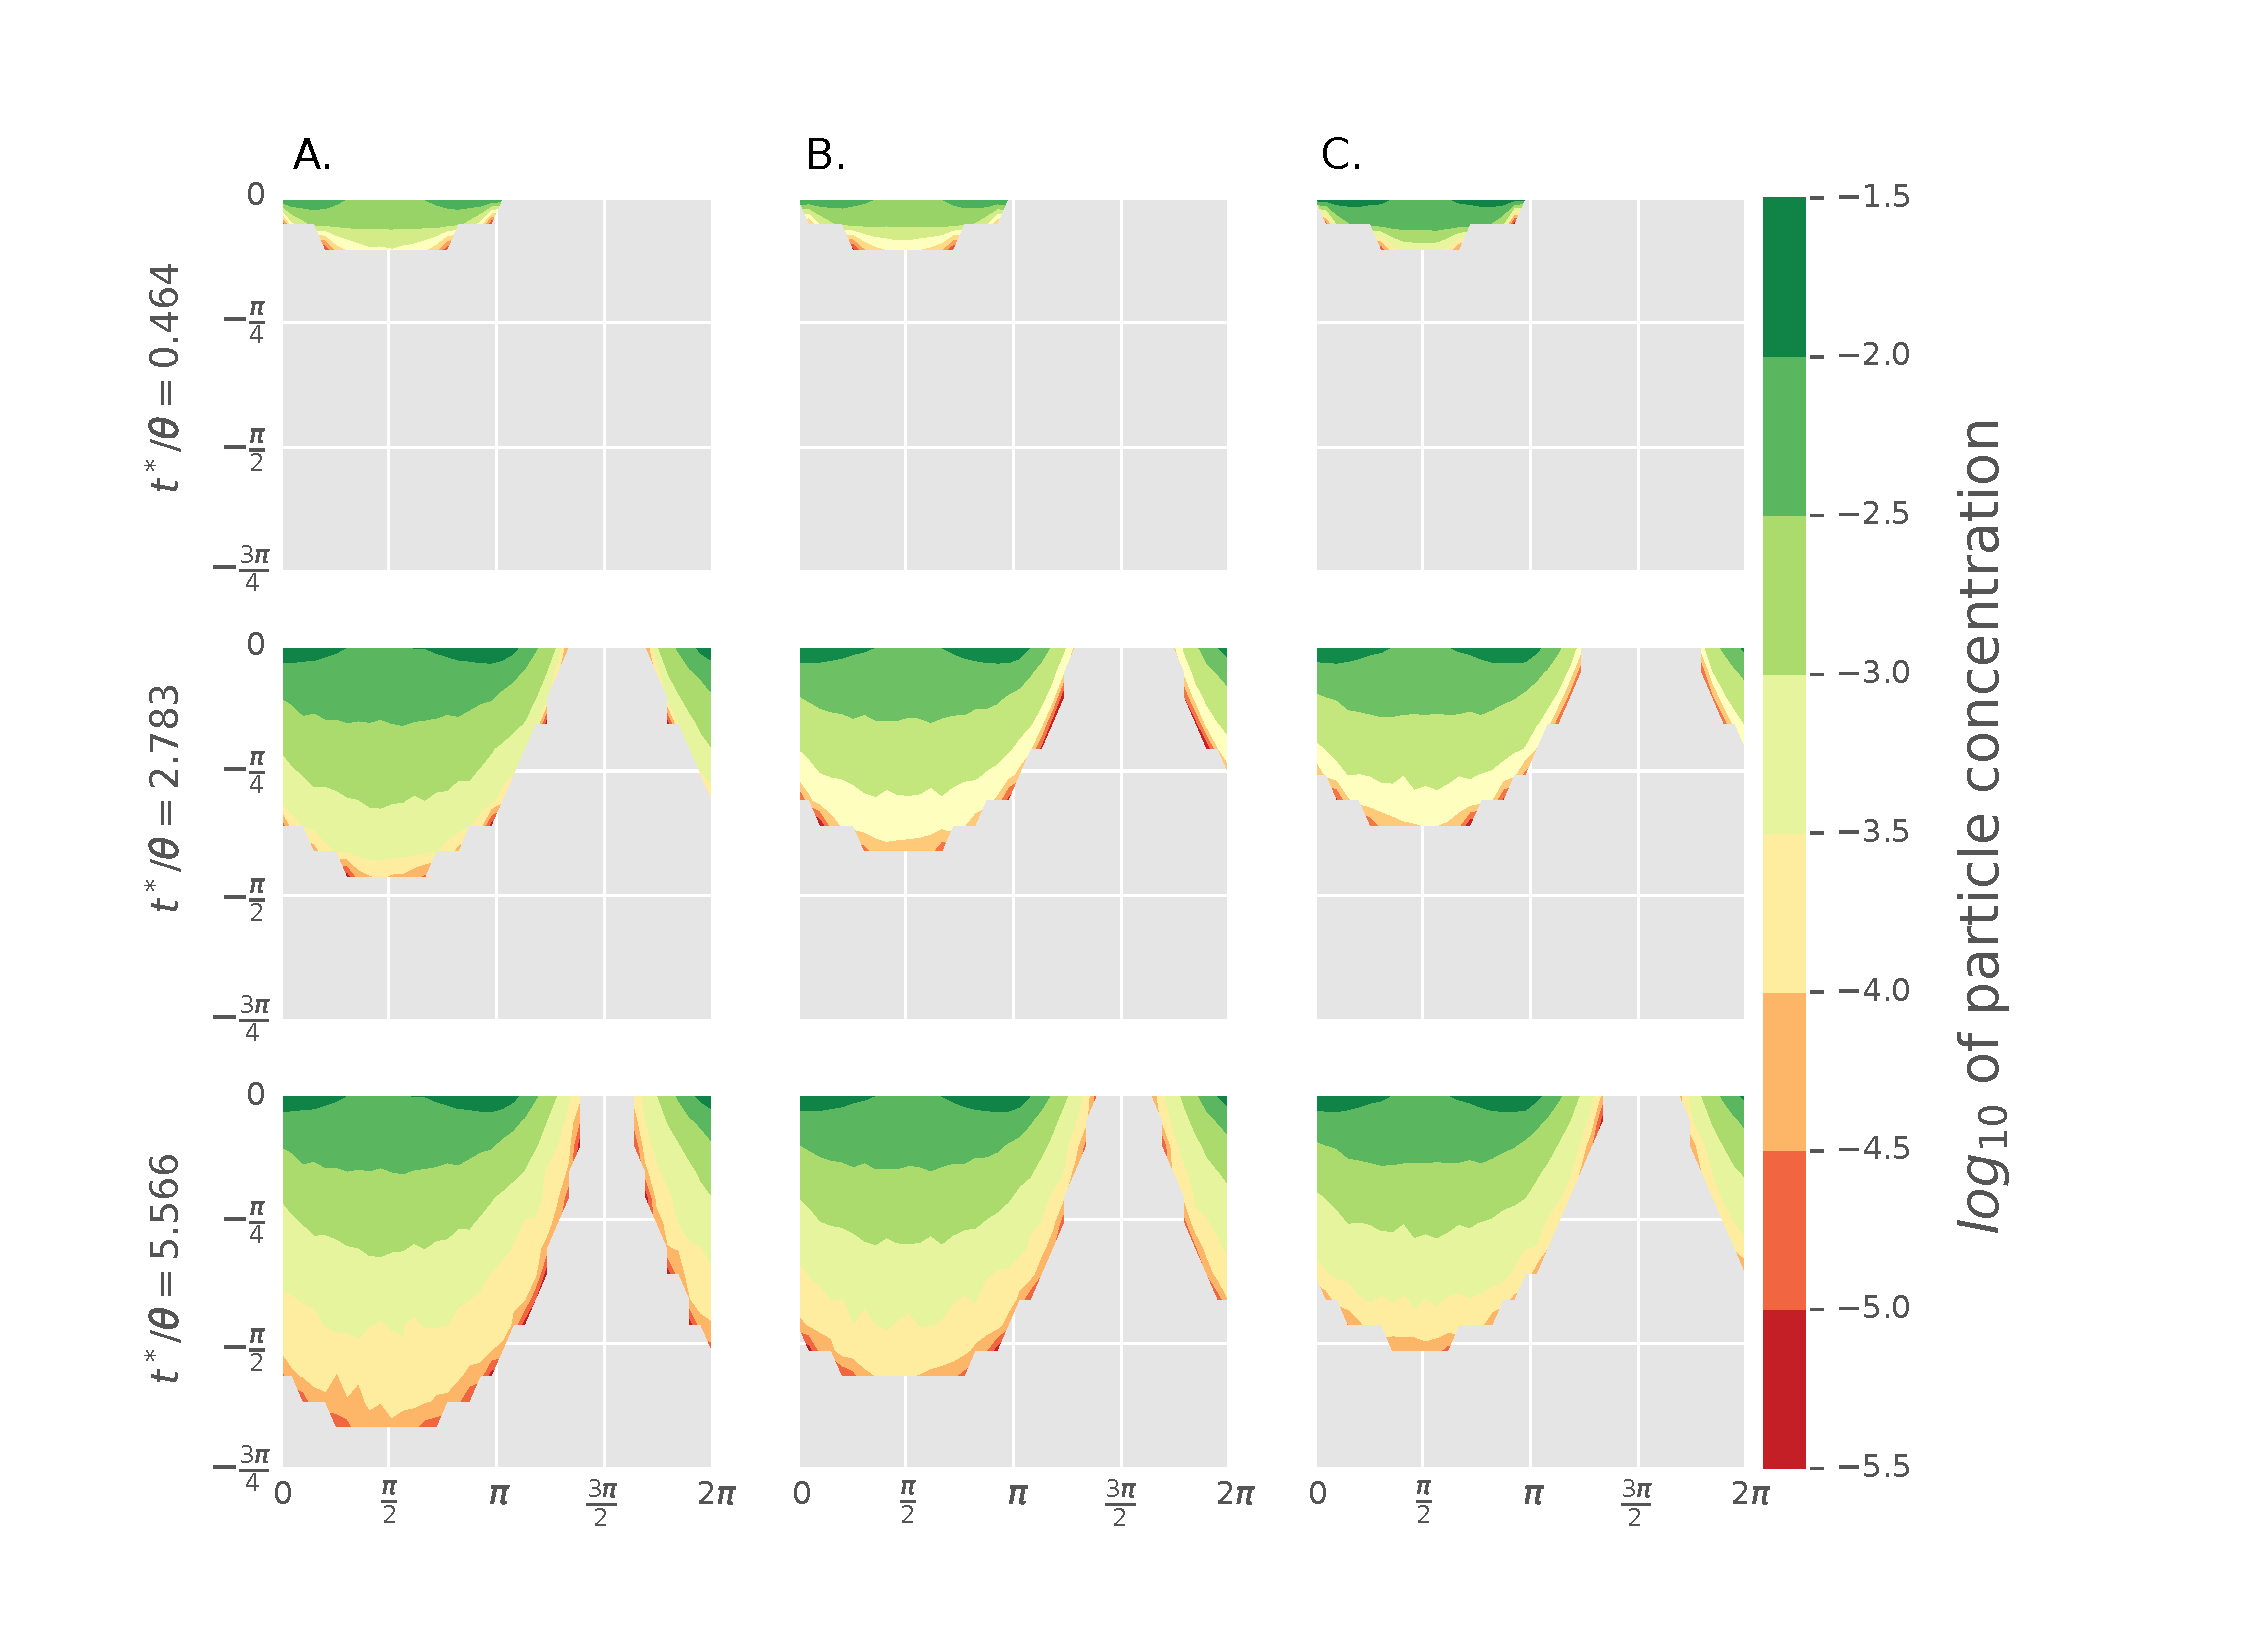
\includegraphics[trim=0.2cm 0.2cm 0.2cm 0.2cm, width=60pc]
{190131_Logplot.pdf}
\caption{Logarithm of particle deposition in different times (rows), and under different inflow/outflow conditions (columns) (Note that axis are not to scale).}
\label{Logmap}
\end{sidewaysfigure}
% ============================================================================

Both, horizontal and vertical extents of the particle deposition are dependent on the vertical flow conditions that are imposed to the numerical model. Fine particles' deposition pattern is similar for early times, though their internal distribution is different between the analyzed cases. For later times, the maximum depth of the clay in all of the times is different between the conditions modeled, similar to the the experimental results used for comparison \citep{Fox2018}. In addition, a particular feature arises near the last quarter of the domain, where a gap is formed and no particles are present even at the top of the domain. This position marks the place where particles go out of the domain and are recirculated to the free surface flow. 

A perceptible difference between particles' deposition can be spotted when analyzing the width the gap formed between the places where particles are deposited. This result is clearly linked to the shape of the velocity profiles and marks the place where particles that are recirculated go out of the domain to the free stream flow. This gap is different in size according to the conditions that are being modeled (figure \ref{Logmap}). Namely, for the losing condition the gap is narrow, and it tend to stretch in neutral and gaining conditions. 

Besides the gap, the logarithmic plot containing the number of particles shows that for the losing condition the amount of particles is more even at the top of the domain than for the neutral and gaining conditions. Besides, the width of the blue strata that shows more than $10^2$ particles is consistent only in the losing condition, while it tends to get thinner in the neutral condition and even tends to disappear for the gaining flow condition.

% 2. BEHAVIOR OF PARTICLES' IN TIME - HOW THEY GET DEPOSITED AND recirculated IN TIME ACCORDING TO THE FLOW CONDITIONS
Regarding the behavior of particles over time (figure \ref{Pvst}), the relative number of particles that are moving inside the domain (figure \ref{Pvst} blue line), filtered (figure \ref{Pvst} purple line) and recirculated to the surface (figure \ref{Pvst} red line). In particular, even with identical filtering coefficients, the amount of particles that remain in the domain and that are recirculated varies significantly betwixt vertical flow conditions imposed.

% ============================================================================
% Particles in time - figure
\begin{sidewaysfigure}
\centering
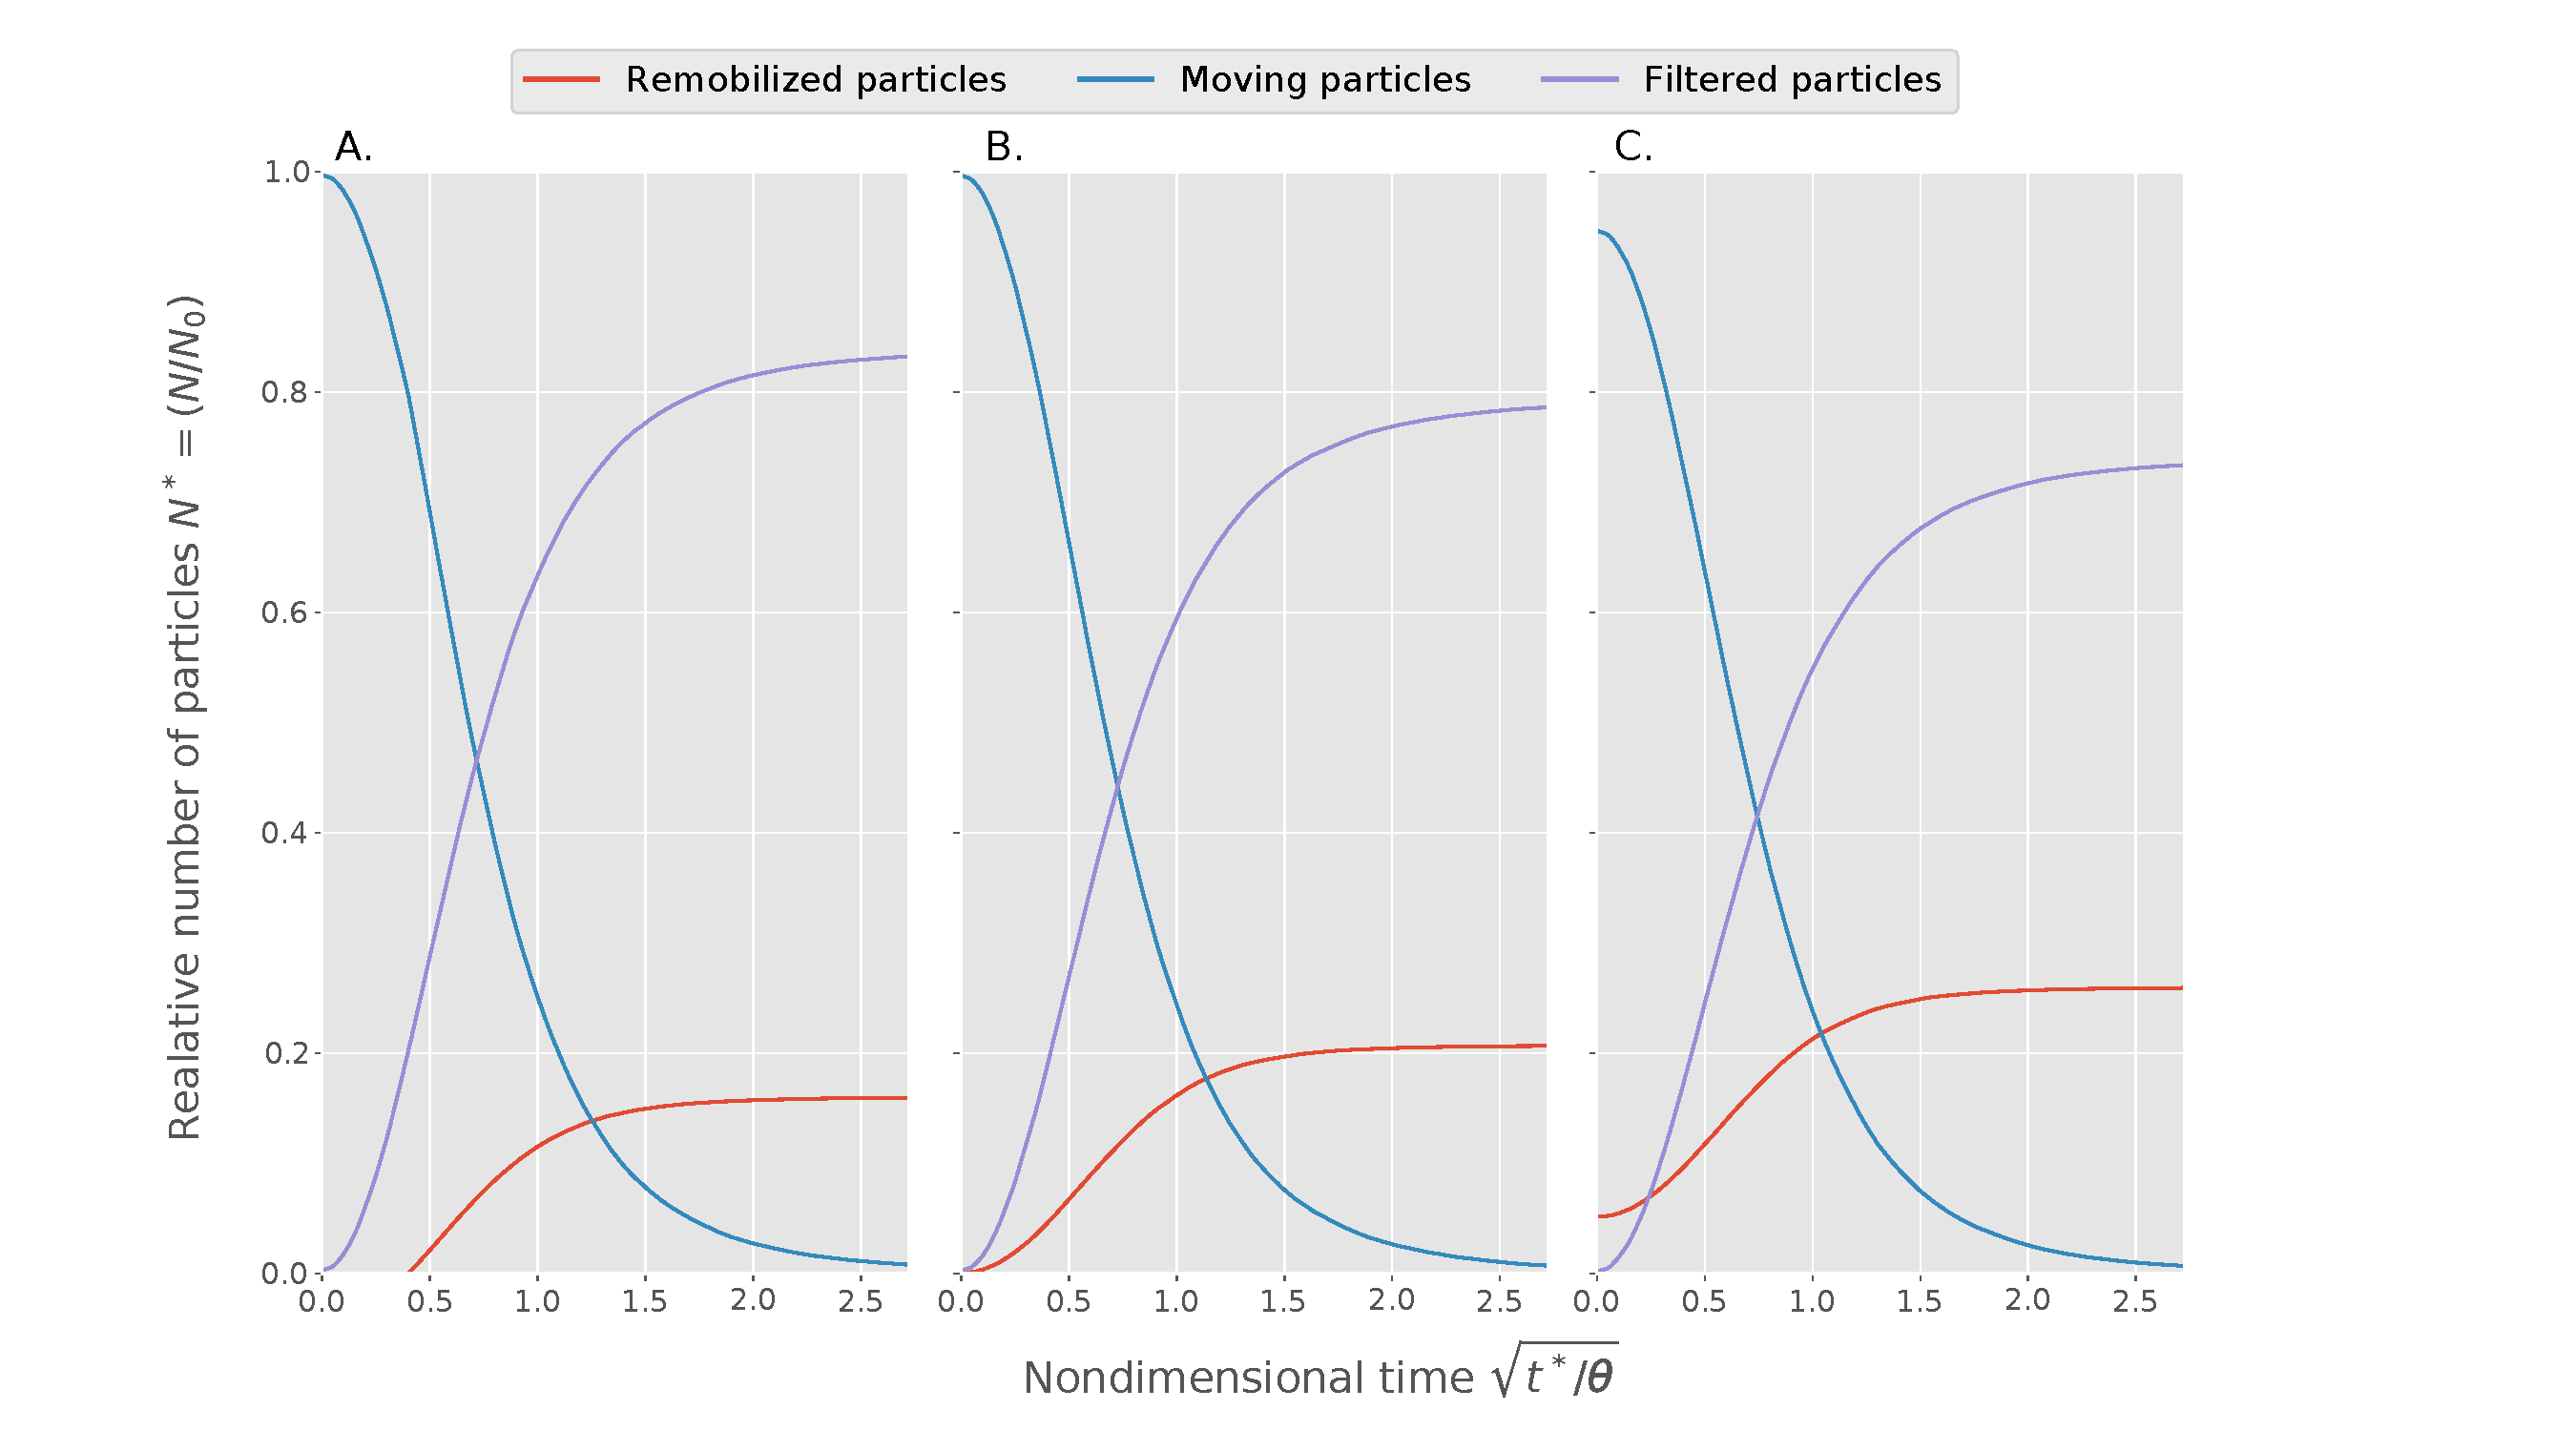
\includegraphics[trim=0.2cm 0.2cm 0.2cm 0.2cm, width=60pc]
{190131_Pvst.pdf}
\caption{Particle's behavior over time. A. Losing condition. B. Neutral condition and C. Gaining condition}
\label{Pvst}
\end{sidewaysfigure}
% ============================================================================

As regards to the moving particles in the domain, it is clear that they decrease in an exponential shape because of the filtering process that is occurring during the time of the simulation in the three modeled scenarios. Indeed, this decrease corresponds to the exponential decrease that results from solving equation \ref{Filt_cont} in a typical filtration problem. Nevertheless, the particles' decrease rate in the domain is different between the different vertical flow conditions showing that the filtering process is fostered or hindered by losing and gaining conditions, respectively. 

In the same way, the number of recirculated particles behaves according to the vertical flux imposed to the model. Therefore, as the flux increases positively (upwards), the number of recirculated particles increase respect to conditions with no vertical or negative (downwards) flux imposed. Distinctly, the number of recirculated particles is high at early times and it decreases as the simulation time goes by, rather than staying constant in time. 

On the subject of filtered particles, vertical flow conditions affect their presence inside the model's domain (figure \ref{Pvst}). Namely, the losing condition fosters the presence of filtered particles, while gaining flow condition hinders it. These results also work in the sense of checking that the sum of filtered, moving and recirculated particles at any time are the total number of particles seeded at the beginning of the simulation. 

% 4. RESIDENCE TIME AND PORTION OF PARTICLES INSIDE THE DOMAIN AT ANY GIVEN TIME.
Besides particles' location in space and time, the PT model can estimate the Residence Time Function (RTF). This feature points the fraction of mass that is present inside the stream bed after and injection performed in a given time $t_0$ \citep{Elliott1997,Packman2000}. Therefore, dividing the the sum of filtered particles and moving particles inside the domain by the total number of particles seeded will result in the RTF of the PT model (figure \ref{RTF}).

% ============================================================================
% Residence time function - figure
\begin{figure}[ht]
\centering
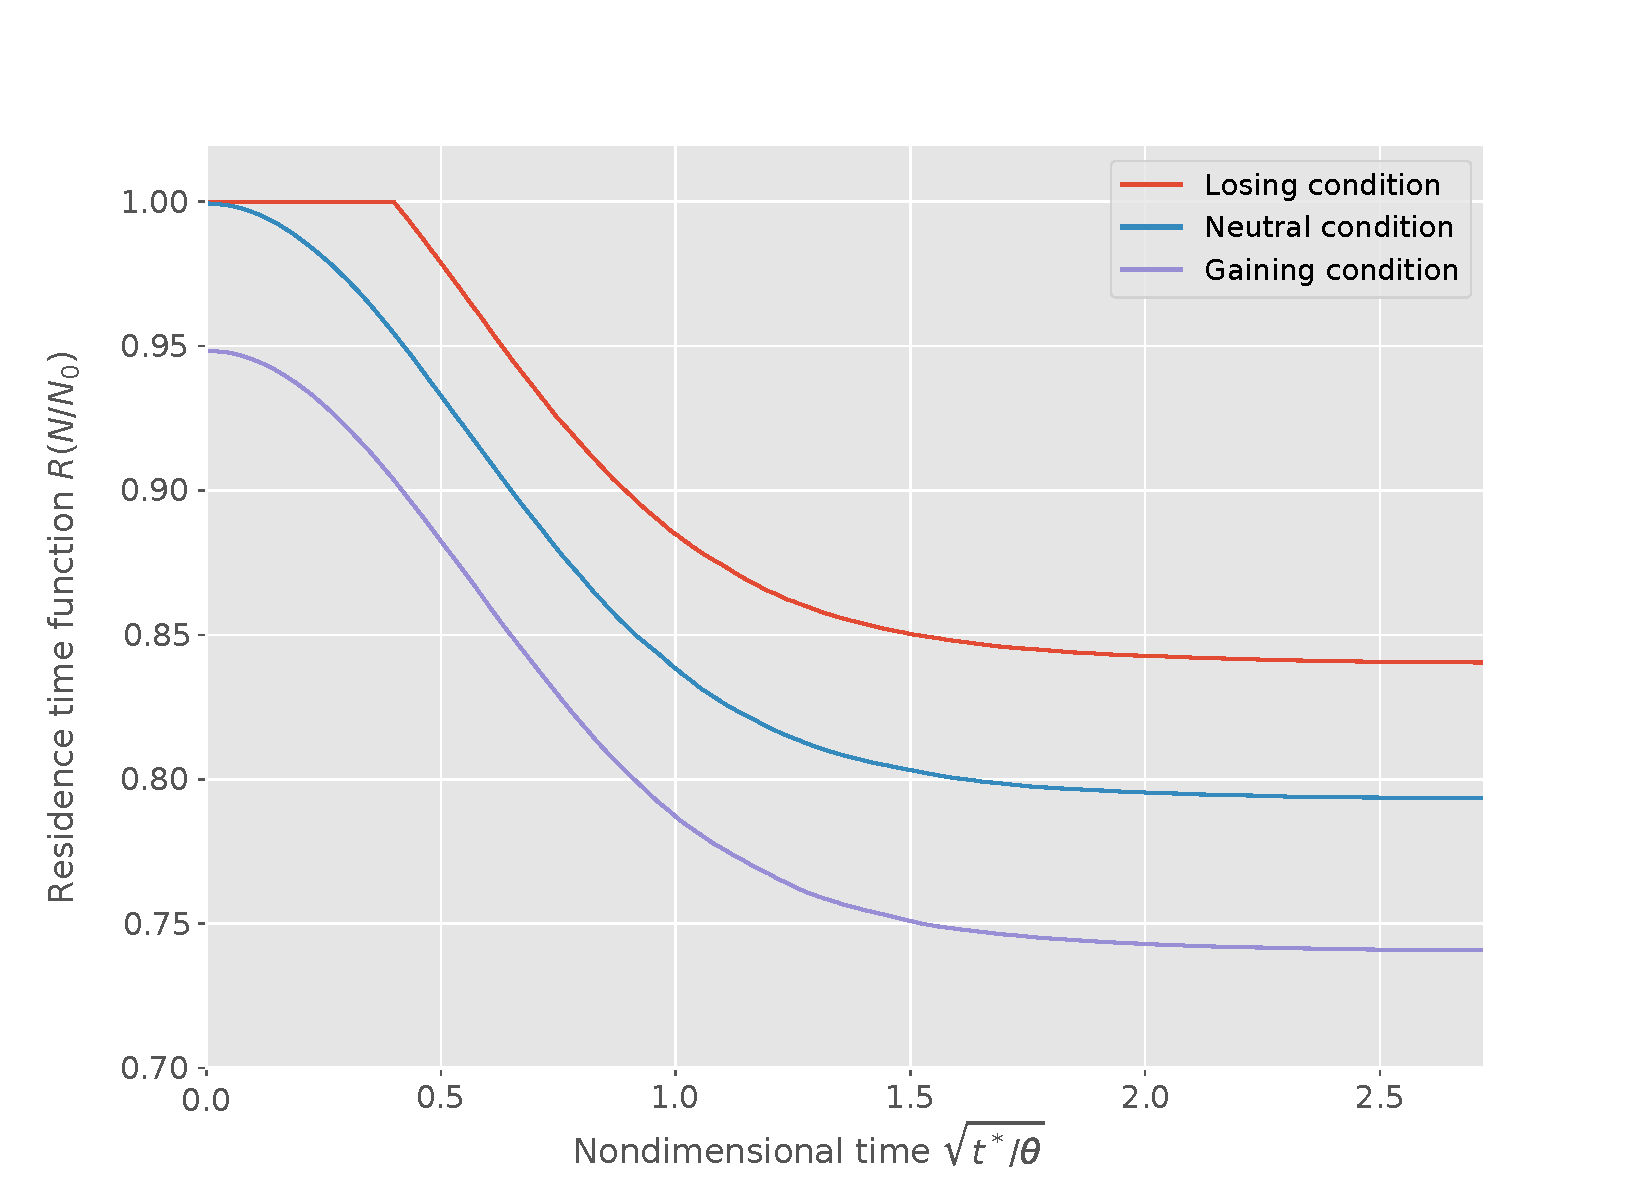
\includegraphics[trim=0.2cm 0.2cm 0.2cm 0.2cm, width=35pc]
{190131_RTF.pdf}
\caption{Residence time function for different flow conditions imposed}
\label{RTF}
\end{figure}
% ============================================================================

% 5. Residence time function and the derivative (check when the othe rmodel is run)
The RTF (figure \ref{RTF}) shows that some of the particles will remain in the bed indefinitely since they have been filtered by the model and cannot be remobilized. Nevertheless, the amount of particles inside it is clearly affected by the vertical flow conditions imposed, since more particles are retained in the bed in the losing condition than in the neutral or in the gaining condition. Furthermore, the RTF is not constant until late times, showing that filtration and vertical flow conditions affect fine particles' deposition.   

Since the gaining and losing conditions are ``symmetrical'', the expected results of the RTF for the losing and gaining conditions are expected to be equally distant from the RTF curve of the neutral condition. Nevertheless, this is not the case. Actually, the losing condition RTF is closer to the neutral condition than the gaining one. To explore this, the rate of change of the RTF in time was estimated for the three cases (figure \ref{RTFder}). To obtain these curves, the gradient of the RTF was taken, and then a moving average with a constant box was performed to smooth the peaks of the function. The derivative of the RTF can be interpreted as the probability density function of particles leaving the domain when recirculating to the flume.

% ============================================================================
% RTF der - figure
\begin{figure}[ht]
\centering
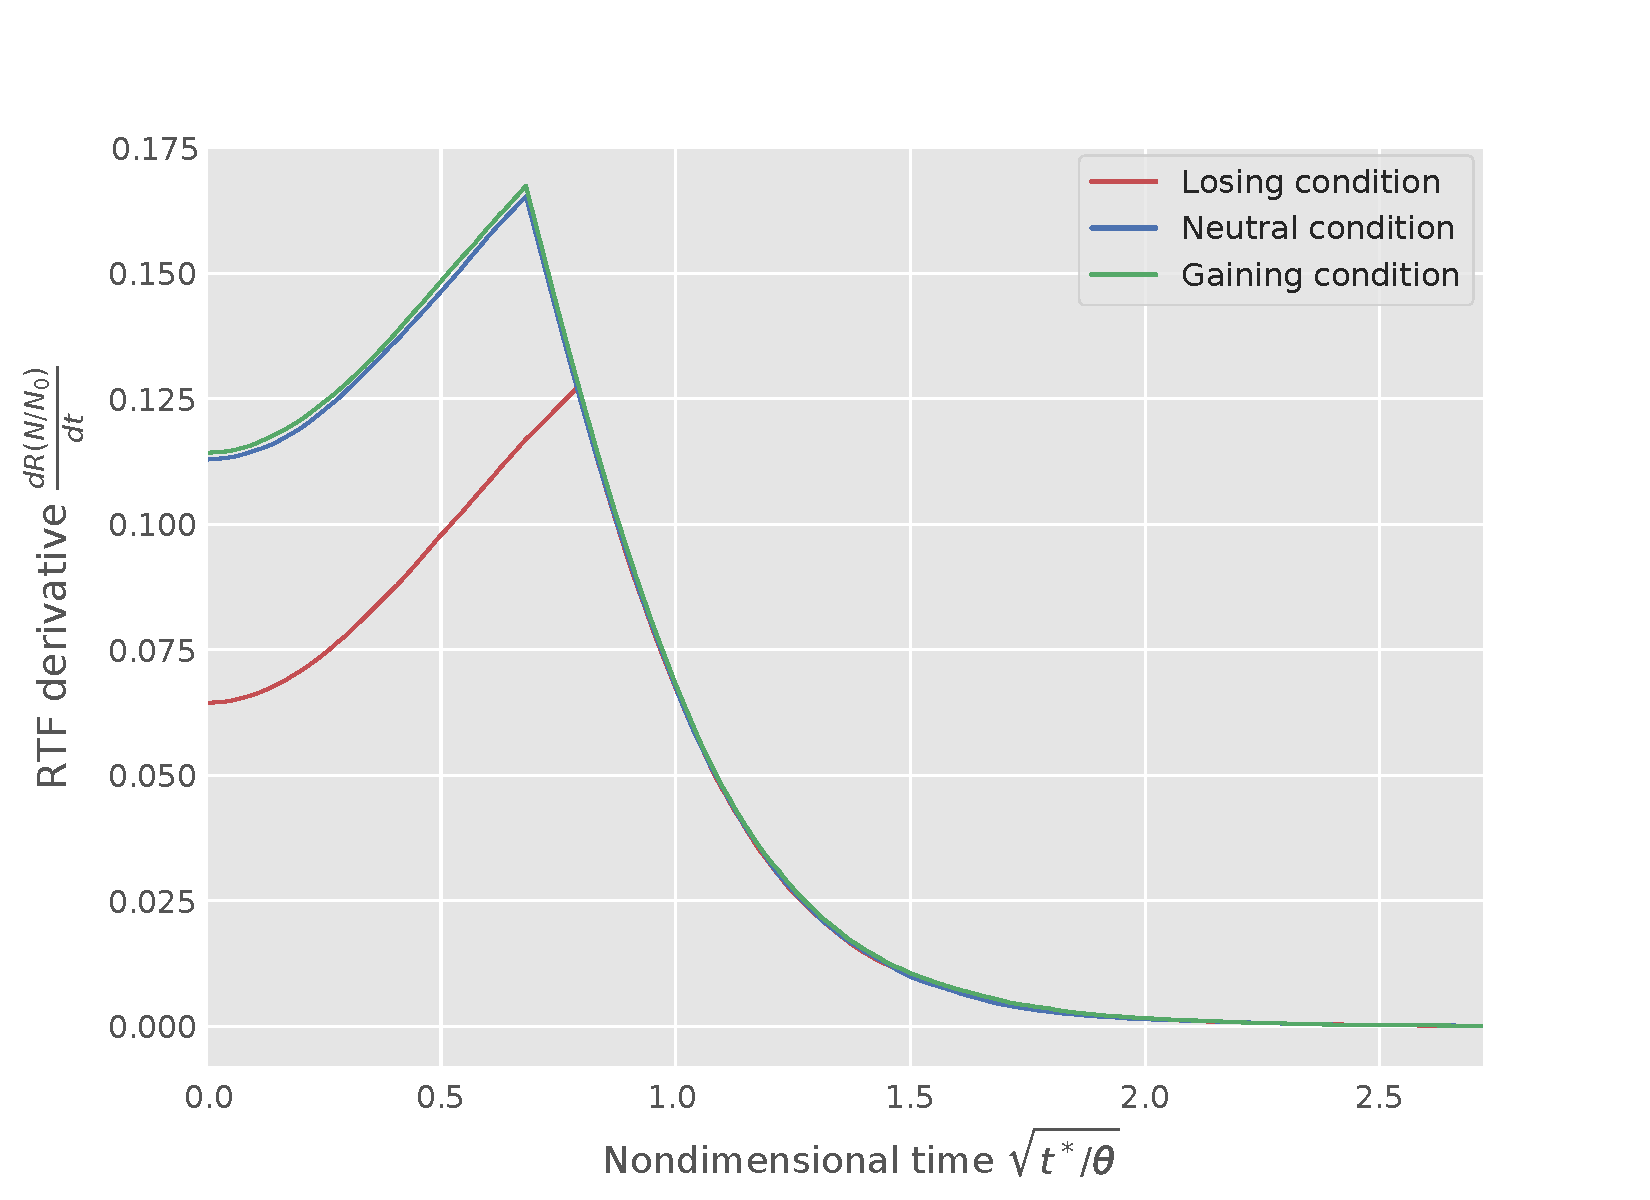
\includegraphics[trim=0.2cm 0.2cm 0.2cm 0.2cm, width=35pc]
{190131_RTF_der.pdf}
\caption{Derivative of RTF for the three conditions}
\label{RTFder}
\end{figure}
% ============================================================================

In addition, for the losing condition all of the particles stay inside the domain for a small time and later they start recirculating (figure \ref{Pvst}), thus the RTF is constant at early times and starts to change after certain time that corresponds to the minimal path that a particle can travel through the domain. The rate of change of the RTF also reflects this feature (figure \ref{RTFder} red line), starting with a lower probability of particles leaving the domain and a maximum probability lower than in the other two conditions modeled. 

It is evident that for any time after the peak probability of recirculation, the rate of change of particles inside the domain is the same for the three conditions modeled (figure \ref{RTFder}). Nonetheless, in the losing condition particles are attracted to stay in the domain more at early times and their probability to leave it is reduced but reaches the other two curves after reaching its peak.

Even so, the three RTF (figure \ref{RTF}), stop changing after a certain time since all of the particles of the domain have been filtered or have left the domain due to recirculation to the free surface flow. Moreover, the fraction of mass remaining inside the domain after any time $t^*/\theta$ is different for each one of the vertical flow conditions modeled. 

% 5. COMPARISON BETWEEN NUMERICAL AND EXPERIMENTAL RESULTS FORM FOX'S PAPER
After observing the numerical model results, they are compared with the experimental results from \citet{Fox2014,Fox2018}. In this work the dunes were divided in four locations, each one corresponding to a quarter part of the dune. Therefore, to compare these results with the model, the non-dimensional domain is divided in sections with $\pi/2$ width. Then, the experimental results estimated the mean and standard deviation of the mass fraction of clay every $0.5cm$ of depth. 

% ============================================================================
% Comparing with experimental results - figure
\begin{sidewaysfigure}
\centering
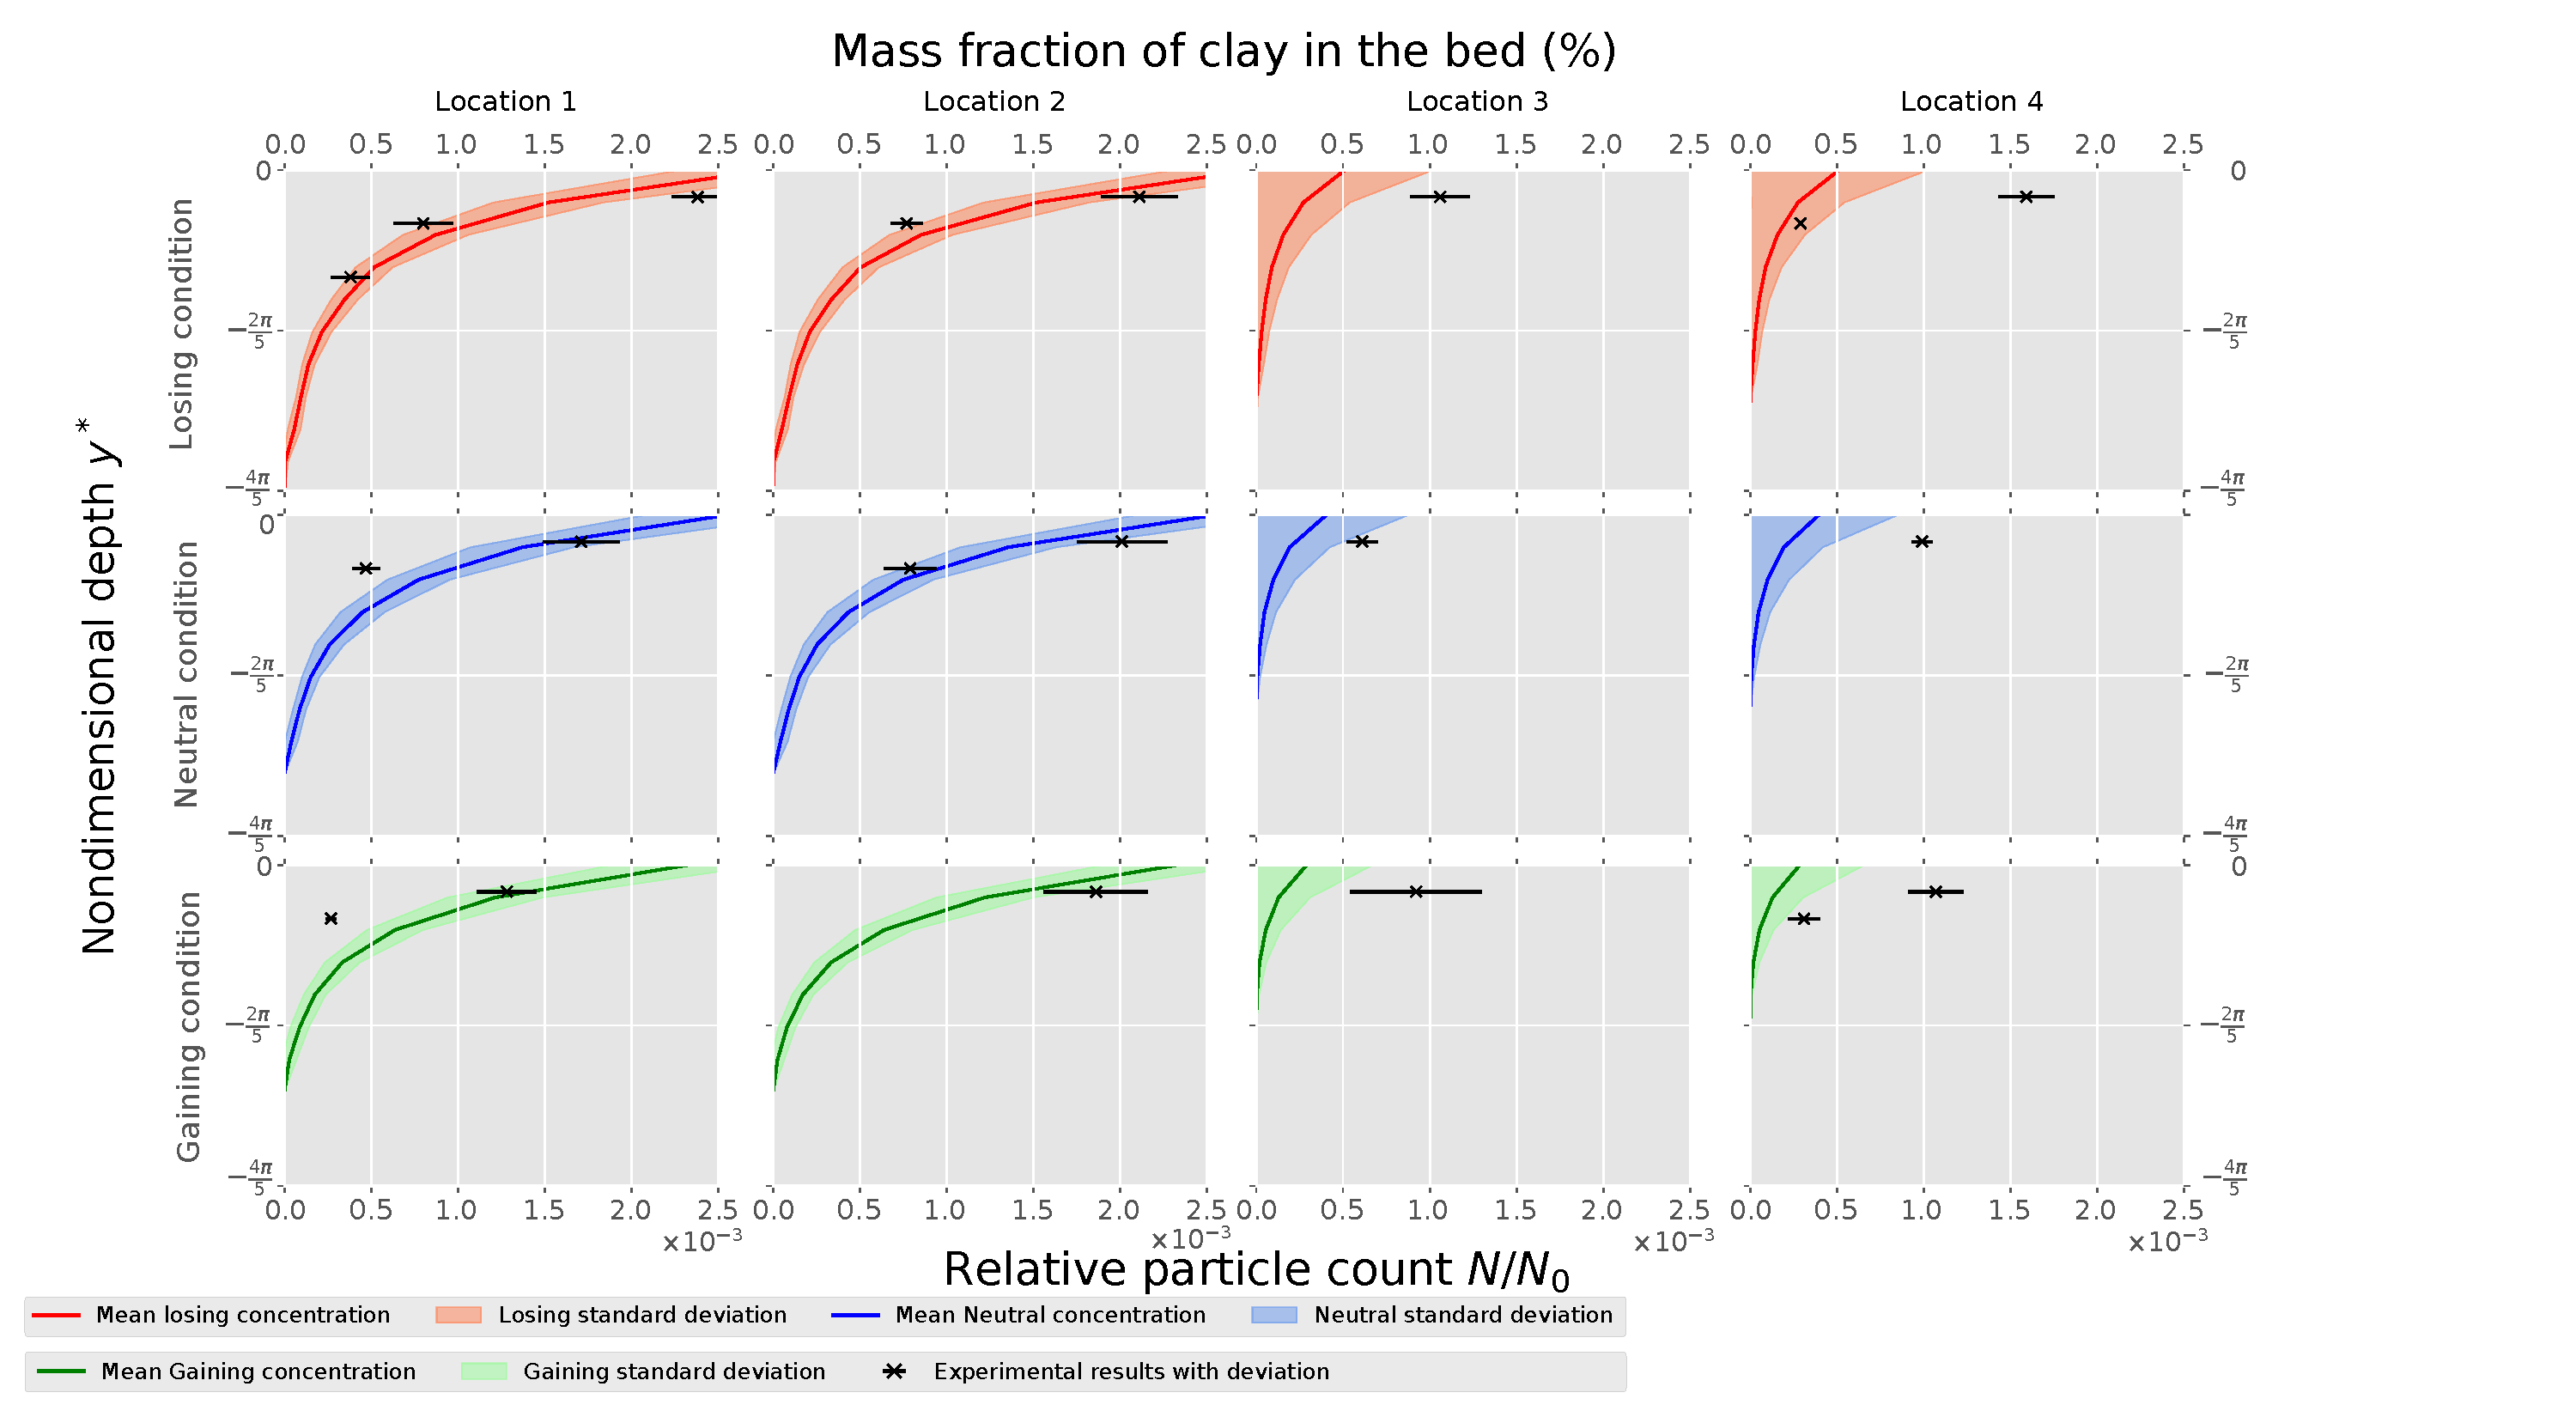
\includegraphics[trim=0.2cm 0.2cm 0.2cm 0.2cm, width=65pc]
{190131_Comparing.pdf}
\caption{Comparison with experimental results from \citep{Fox2018}}
\label{Comparison}
\end{sidewaysfigure}
% ============================================================================

Our model's results are compared qualitatively with the aforementioned experimental results (figure \ref{Comparison}). Black crosses show the mean mass fraction in the depth of reference, and its lines show the plus or minus standard deviation. The scale for these results is shown at the top of figure \ref{Comparison} and it is represented by the percentage of clay mass over total mass of the core extracted. 

Similarly, the colored lines in figure \ref{Comparison} show the mean relative number of particles and the shading shows the standard deviation of this quantity. The scale is located in the bottom part of figure \ref{Comparison} and it is different than the one used for the experimental results. Nonetheless, both shapes are similar and in a quantitative sense they look similar for the experimental and numerical experiments.

Moreover, clay deposition varies according to the location that is analyzed. In other words, clay tends to deposit more in locations one and two (the stoss side of the dune), and reduces its deposition in locations three and four (lee side of the dune). In fact, the deposition in the latter is provided by the particles that move from right to left in the computational domain following the path lines (figure \ref{Velocities}).

Nevertheless, our results show that at locations three and four the PT model is not as good as in locations one and two. For all of the three cases modeled, the experimental results show more clay over depth for locations three and four (\ref{Comparison}). That is to say, in the experiments more clay is found inside the domain at the lee side than in the PT model. 

All in all, our results show that there are notable differences between the cases modeled that represent the physics of clay deposition for the conditions imposed. However, the similarities of the PT model with the experimental results are able to highlight the contribution of filtration and vertical flow to understand the aforementioned process. 

% ================================================================================
% DISCUSSION SECTION
% ================================================================================
\section{Discussion} \label{Discussion}

% 1. Velocity profiles and deposition patterns analyzed
The proposed PT model combines the use of Langevin's equation and a stochastic filtration framework \citep{Li2017} to simulate fine particles' deposition in a generalized condition. Indeed, its formulation is simple and straightforward. Moreover, this model does not pose any problems regarding mass conservation, artificial diffusion or unwanted oscillations provoked by numerical scheme instabilities \citep{Delay2005}. For the present research, the model was used to assess fine particles' deposition with static dunes and different vertical flows imposed. 

Although the surface flow conditions are the same, the change in vertical flow conditions reshape the streamlines that are followed by the model's particles. Actually, the Stokes number of an individual particle is so low that it is safe to assume that they stick perfectly to the streamlines generated by the velocity profiles. In particular, this assumption is made because of the size of a typical clay particle and the maximum velocity which it is subject to when entering the streambed that is being modeled. 

Stokes number is defined as the relation between the stopping distance and the characteristic length of the phenomenon \citep{Clark2009}. For our model, it was shown in sub subsection \ref{Mathematical_model}. Consequently, the phenomenon of settling velocity inside the sand bed is not taken into account as it was in previous works \citep{Packman2000}.

Nevertheless, the PT model is able to capture the basic physics of the problem. Namely, the velocity profiles and the deposition patterns show that there are important differences between the conditions modeled (figures \ref{Velocities} and \ref{Logmap}). In fact, the gaining flow condition produces less deposition than the neutral and losing condition. Also, for the three conditions, deposition is present only at the top of the domain, showing that the model's depth is not relevant for the phenomenon of clay deposition since it deposits at the top and there is no particle penetration to deep parts of the domain. 

Moreover, the logarithmic deposition patterns (figure \ref{Logmap}), show that a change in the vertical flow conditions affect not only the maximum penetration depth of the particles, but also spread more evenly in the horizontal direction. In that sense, particles' presence in the streambed will cover more dune's width in the losing condition and it will be discontinuous in the neutral and gaining cases. In effect, this explains the decay hyporheic exchange in the experiments run with conservative tracers after clay injections under different vertical flow conditions \citep{Fox2014,Fox2018}.

In addition, the PT model shows that the velocity profiles and filtration produce an uneven distribution of particles in horizontal layers. In other words, clay penetration is stratified, but these layers are not constant over the domain but will locate in ``preferential'' places. as a consequence, our results suggest agreement with experimental results that clearly show an uneven distribution of clay mass in the dunes where the cores were extracted \citep{Fox2018}.

As respects to the comparison made with the experiments (figure \ref{Comparison}), our results suggest that the PT model is able to simulate clay deposition in an idealized dune with similar results to the experiments. Indeed, the decay in clay concentration with depth is similar to the experimental results presented by \citet{Fox2018}, suggesting that the PT model grasps the physical processes of clay deposition in sand beds. However, regarding the standard deviation of clay's mass fraction is not as accurate as expected. This can be explained by the difference in shape of the dunes in the experiment and the proposed dune for the numerical model. On one hand, for the experimental set up, the shape of the dunes and the material porosity are not homogeneous because of the normal conditions of the experiment. On the other hand, our model simulates and idealized dune with a fixed shape and constant physical properties inside the domain.   

% 2. Discussion about the particle's behavior over time (remobiliztion, RTF and what does that imply in the context of clay deposition)
Regarding the behavior of particles over time, the differences between vertical flow conditions are also noticeable in figures \ref{Pvst} and \ref{RTF}. For example, particles tend to be recirculated easily when there is the presence of a gaining flow. Total recirculated particles between cases ranges from 0.18 in the losing condition to almost 0.3 in the gaining scenario (units in fraction of particles). Namely, recirculated particles almost double when passing from the losing to the gaining case. This result suggests that the particles' concentration decay in a flume with a constant and well mixed supply of sediment will be lower for gaining conditions than for neutral or losing conditions, as shown by \citet{Fox2018}.

In particular, for the particles' filtering, our results suggest that the vertical flow conditions play a crucial role in affecting this process. Granted that the filtering coefficient is the same for all of the modeled scenarios, particle filtering is fostered by losing flow conditions. That is, the more negative the vertical velocity is, the more a particle is going to travel inside the streambed, and therefore will be more prone to be subject to filtering during the simulation. 

Furthermore, the rate of change of the RTF (figure \ref{RTFder}) suggests that the particles' movement and retention inside the domain depends also on the imposed flow conditions and not just on the filtration coefficient. The RTF curves (figure \ref{RTFder}) suggest that the filtration process is the same for all of the modeled cases and that the initial remobilization caused by the imposed flow condition is the main driver of the phenomenon analyzed. 

Consequently, in all of the cases the main difference is set at the initial times of the simulations, where particles are recirculated according to the imposed vertical velocity. In fact, particles that are not recirculated at early times are subject to movement or filtration, and the more particles are moving inside the domain (losing condition), the more the filtration process will act during the simulation. 

In general, our model shows that clay deposition is a phenomenon that results from the combination of the velocity inside the streambed, the vertical flow condition (losing, neutral or gaining), and the filtering properties of the material. In order of importance, the filtering part of the model enforces the stopping of clay particles inside the porous matrix. However, this process is fostered and changed drastically when a vertical flow is imposed. 

% ================================================================================
% CONCLUSIONS SECTION
% ================================================================================
\section{Conclusions} \label{Conclusions}

The PT model implemented and presented in this paper combines the physical description of the fine sediments' movement with the probabilistic framework of particles' filtration inside a characteristic sand dune. Moreover, our model presents a novel approach that pretends to be a generalization of sediment movement in any given sand dune with free surface and groundwater flow conditions known. Therefore, when it is combined with a strong and simple numerical framework it can represent the mean behavior of fine sediments' deposition in natural systems. 

Namely, these models are more suitable to represent phenomena that is not described accurately with the ADE \citep{Noetinger2016}. Moreover, their results are straightforward to interpret since all of the calculations are made with the number of particles inside the computational domain, and the operations performed to obtain the results are numerous but not complex and there is no mesh for discretizing the physical domain, as in typical schemes like finite element, volumes or differences.

Indeed, when comparing our model with traditional schemes, mass conservation is ensured at all time, there is no artificial diffusion (especially numerical diffusion), and the results are comparable with experimental set-ups from previous works. Nonetheless, this numerical simulation can assess different results and highlight important features that the experiments cannot recognize or fail to assess due to inherent heterogeneity and lack of parameters' control. For instance, if a flume uses a detemrined type of sand, both the dunes' shape and the porosity (hence, the permeability), are not going to be homogeneous in all of the domain. Therefore, our model is suitable to represent idealized media and explain mean results of the pehnomena captured. 

Regarding these features, our model shows clearly that the vertical flow conditions imposed are responsible for the differences in deposition patterns and amount of clay inside the domain. Similarly, the filtration phenomenon will act as a control of particles inside the domain. Consequently, when in the presence of gaining flow condition, the amount of particles inside the domain will be less than in the other two cases, while the rate at which particles are filtered inside the domain is the same for all of the three modeled cases.

In particular, our model's most important finding is that vertical flow condition affects particles' deposition regardless of the filtration phenomenon inside the domain. Therefore, the differences in deposition patterns, maximum penetration depth and the steady final value of the RTF are caused mainly by vertical velocities imposed as losing/gaining conditions. On the other hand, filtration coefficient is responsible for the time that takes to the RTF to get to a constant value after the first injection. Put differently, vertical flow conditions imposed relocate particles and recirculate particles out of the domain in different amounts and account for the difference between the three cases modeled.

As regards to particles' recirculation to the free surface flow, this phenomenon is relevant only for a brief time of every one of our models, but its presence and the return of particles from the SWI to the free stream clearly depend also on the vertical flow conditions imposed. In other words, recirculation to the stream is not connected with filtration, but it rather works side by side with it to determine the shape of the residence time function for the different cases modeled. 

However, our model is not able to represent fully the experimental conditions due to structural differences between the PT model and the flume set up. Mainly, our model estimates deposition in a homogeneous media and it does not affect the porosity of the bed, while clearly this physical property is affected with the deposition phenomenon. Furthermore, physical experiments are not perfect, heterogeneity in physical properties and variables like flow and concentration can only be controlled to some extent. Consequently, further work will aim to improve the results of the PT model implemented.

In the direction of testing further our numerical PT model, more experimental results are needed to assess it. In addition, future work aims to represent changes in porosity due to clay's deposition since it is evident that an important clay deposition will hinder flow in specific places and consequently the flow field will change with time due to changes in the hydraulic conductivity of the media. 

To conclude, the PT framework is suitable to study phenomena that is difficultly modeled by continuum mechanics equation such as ADE. Their flexibility allows to model phenomena in small scale $O(10^{-1}m)$ to reach scale $O(10^3-10^4 m)$ with results that are comparable to experimental or field study results.  

\acknowledgments
We thank Zuckerberg Institute for Water Research, The J. Blaustein Institutes for Desert Research, Ben-Gurion University of the Negev (Beersheba, Israel), for providing the experimental data for comparisons; and the Water Research Group at Northwestern University for providing the basis for the particle-tracking model. This research was funded by Colciencias grant 647; the James W. Fulbright Association under the program of visiting doctoral student; the HERMES mobility system of Universidad Nacional de Colombia. Supporting information codes are available at (FIGSHARE\_URL). Authors declare no conflicts of interest.

% References and Citations
\bibliography{Paper_PT.bib}

% % FIGURE IN THE END OF THE DOCUMENT TO MATCH DRAFT SUBMISSION

% % ============================================================================
% % Conceptual model of the problem proposed - figure
% \begin{figure}[ht]
% \centering
% \includegraphics[clip, trim=4.2cm 4.5cm 8cm 3cm, width=18pc]
% {1807010Conceptual.pdf}
% \caption{Conceptual model for the posed problem}
% \label{Conceptual}
% \end{figure}
% % ============================================================================

% % ============================================================================
% % Velocity profiles - figure
% \begin{figure}[ht]
% \centering
% \includegraphics[trim=2cm 1.5cm 4cm 0.1cm, width=25pc]
% {181203_Streamlines.pdf}
% \caption{Streamlines under different vertical flow conditions: (A) Losing, (B) Neutral and (C) Gaining. Plots' domains are shifted from $[0, 2 \pi]$ to $[-\pi /2, \pi/2]$ since domain is periodic. Note that the vertical scale is distorted.}
% \label{Velocities}
% \end{figure}
% % ============================================================================

% % ============================================================================
% % Numerical model of the problem proposed - figure
% \begin{figure}[ht]
% \centering
% \includegraphics[clip, trim=4.2cm 4.5cm 8cm 3cm, width=18pc]
% {181129Numerical.pdf}
% \caption{Depiction of numerical model proposed}
% \label{Numerical}
% \end{figure}
% % ============================================================================

% % ============================================================================
% % Concentration map - figure
% \begin{figure}[ht]
% \centering
% \includegraphics[trim=0.2cm 0.2cm 0.2cm 0.2cm, width=45pc]
% {181203_Concentrations.pdf}
% \caption{Particle deposition in different times (rows), and under different inflow/outflow conditions (columns) (Note that axis are not to scale).}
% \label{Heatmap}
% \end{figure}
% % ============================================================================

% % ============================================================================
% % Logarithm of concentration - figure
% \begin{figure}[ht]
% \centering
% \includegraphics[trim=0.2cm 0.2cm 0.2cm 0.2cm, width=45pc]
% {181203_Logplot.pdf}
% \caption{Logarithm of particle deposition in different times (rows), and under different inflow/outflow conditions (columns) (Note that axis are not to scale).}
% \label{Logmap}
% \end{figure}
% % ============================================================================

% % ============================================================================
% % Particles in time - figure
% \begin{figure}[ht]
% \centering
% \includegraphics[trim=0.2cm 0.2cm 0.2cm 0.2cm, width=35pc]
% {181203_Pvst.pdf}
% \caption{Particle's behavior over time. A. Losing condition. B. Neutral condition and C. Gaining condition}
% \label{Pvst}
% \end{figure}
% % ============================================================================

% % ============================================================================
% % Residence time function - figure
% \begin{figure}[ht]
% \centering
% \includegraphics[trim=0.2cm 0.2cm 0.2cm 0.2cm, width=20pc]
% {181203_RTF.pdf}
% \caption{Residence time function for different flow conditions imposed}
% \label{RTF}
% \end{figure}
% % ============================================================================

% % ============================================================================
% % RTF der - figure
% \begin{figure}[ht]
% \centering
% \includegraphics[trim=0.2cm 0.2cm 0.2cm 0.2cm, width=20pc]
% {181203_RTF_der.pdf}
% \caption{Derivative of RTF for the three conditions}
% \label{RTFder}
% \end{figure}
% % ============================================================================

% % ============================================================================
% % Moving der - figure
% \begin{figure}[ht]
% \centering
% \includegraphics[trim=0.2cm 0.2cm 0.2cm 0.2cm, width=20pc]
% {181203_Moving_der.pdf}
% \caption{Derivative of moving particles inside the domain}
% \label{MOVder}
% \end{figure}
% % ============================================================================

% % ============================================================================
% % Comparing with experimental results - figure
% \begin{figure}[ht]
% \centering
% \includegraphics[trim=0.2cm 0.2cm 0.2cm 0.2cm, width=40pc]
% {181203_Comparing.pdf}
% \caption{Comparison with experimental results from \citep{Fox2018}}
% \label{Comparison}
% \end{figure}
% % ============================================================================

\end{document}